%Latex Template (Master file)
% By Chetan Kandarkar : modified on 14th May 2021.
% Pl. note : this template is used for practice and to show the different functions of LaTeX. Refered citations are not actuals.
%-------------------------------------------------------------
%--------------------------------------------------------------
%Pl. refer the  database.bib file in the folder for references list
% study the syntax for refernces as shown in database.bib

%--------------------------------------------------------
%--------------------------------------------------------
% To create list of table  --
% Run the code twice (pdflatex or latex)
%%%%%%%%%%%%%%%%%%%%%%%%%%%%%%%%%%%%
%To get the references using bibtex follow following sequence.
%pdflatex
%bibtex
%pdflatex
%pdflatex
%%%%%%%%%%%%%%%%%%%%%%%%%%%%%%%%%%%%%%%%%%%%%%%%%%%%%
%%%%%%%%%%%%%%%%%%%%%%%%%%%%%%%%%%%%%%%%%%%%%%%%%%%
\documentclass[12pt,a4paper,final,oneside]{report}

\usepackage{geometry}
\usepackage{amsfonts}
\usepackage{amssymb}
\usepackage{graphics}
\usepackage{graphicx}
\usepackage{amsmath}
\usepackage{array}
\usepackage[pdftex]{hyperref}
\usepackage{epstopdf}
\usepackage{setspace}
\usepackage{natbib}


\begin{document}

\thispagestyle{empty}
%%% This is first page
%%%%% Refer q31.tex file



\begin{center}
	
	\LARGE \textbf  {IoT based Smart Sanitizer Dispenser}
	
\end{center}
\vspace{0.2cm}


\begin{center}
	
	 {Submitted in partial fulfilment of the requirements} \linebreak {Of the degree of}
	\vspace{0.2cm}
	\linebreak \textbf {Bachelors of Engineering by:}
	
\end{center}
\vspace{0.2cm}
\begin{center}
	
	\textbf{Chetan Kandarkar}
	\linebreak \textbf{Monish Soni}
	\linebreak \textbf{Mitesh Vaidya}
	\linebreak \textbf{Sarvesh Shukla}
	\vspace{1cm}
	
	Project Guide:
	\linebreak \textbf{Mr.Mohd Farhan}
\end{center} 
%\vspace{0.2cm}
\begin{center}
	%\begin{figure}[h]
	%	\centering
	
\includegraphics[width=30mm,scale=1]{11}
	%	\label{bbb}
	%\end{figure}\newline
\end{center}

\begin{center}
	\vspace{0.5cm}
	
	\textbf{LOKMANYA TILAK COLLEGE OF ENGINEERING}
	\vspace{0.2cm}
	\linebreak{Affiliated to}
	\vspace{0.2cm}
	\linebreak  \textbf {UNIVERSITY OF MUMBAI}
\end{center}
\vspace{0.2cm} 

\begin{center}

\includegraphics[width=30mm,scale=1]{22}


%\label{fig:mumbaiuni}
\end{center}
\begin{center}
	\textbf {Department of Electronics \& Telecommunication Engineering}
	\vspace{0.1cm}
	\linebreak \textbf {2020-2021}
\end{center}

\newpage
\pagestyle{plain}
\onehalfspacing
%%%%%%%%%%%%%% this is for certificate, pl modify according to your need
% refer q31.tex

\newpage
\thispagestyle{empty}
\begin{center}
\LARGE \textbf { {Certificate} }
\end{center}


\vspace{0.5cm}
This to certify that the project entitled  \textbf{\textquotedblleft IoT based Smaert Sanitizer Dispenser\textquotedblright} is a bonafide work of \textbf{\textquotedblleft Chetan Kandarkar, Monish Soni, Mitesh Vaidya, Sarvesh Shukla\textquotedblright} submitted to the University of Mumbai in partial fulfillment of the requirement for the award of the degree of \textbf{\textquotedblleft Bachelor of Engineering\textquotedblright} in  \textbf{\textquotedblleft Electronics and Telecommunication Engineering\textquotedblright}. 
\vspace{6cm}

\begin{flushleft} \textbf
{Mr.Mohd Farhan} \hspace{10.00mm} \textbf{Dr.Ravindra Duche}\hspace{15.00mm}\textbf{Dr.Vivek Sunnapwar}  \newline



    (Project Guide)  \hspace{18.00mm} (Head of Department) \hspace{22.00mm}
         (Principal)                            
\end{flushleft}











\input{Project.tex}

\newpage
\thispagestyle{empty}
\begin{center}
	\LARGE \textbf  {{Declaration}} 
\end{center}

\vspace{1.00cm}	
	We declare that this written submission represents our ideas in our own words and where others' ideas or words have been included, we have adequately cited and referenced the original sources. We also declare that we have adhered to all principles of academic honesty and integrity and have not misrepresented or fabricated or falsified any idea/data/fact/source in my submission. We understand that any violation of the above will be cause for disciplinary action by the Institute and can also evoke penal action from the sources which have thus not been properly cited or from whom proper permission has not been taken when needed. 
	
	\vspace{2.00cm}
	\begin{flushright}
		\begin{large} \textbf{ Students Name}\end{large} \hspace{20.00mm} \begin{large}\textbf{Signature}\end{large}
	\end{flushright}
	
	\begin{flushleft}	 
	\hspace{60.00mm} \vspace{0.3cm} \textbf{1.Chetan Kandarkar} 
		\vspace{0.3cm}
	\hspace{60.00mm} \textbf{2.Monish Soni}
		\vspace{0.3cm}
	\hspace{60.00mm} \textbf{3.Mitesh Vaidya} 
		\vspace{0.3cm}
	\hspace{60.00mm} \textbf{4.Sarvesh Shukla}
		\vspace{0.3cm}	    
	\end{flushleft} 
	 


\newpage
\pagestyle{plain}
\pagenumbering{roman}
\newpage
%\thispagestyle{empty}
\begin{center}
\LARGE\textbf	{Acknowledgement} 
		
\end{center}

\vspace{2cm} 

We would like to take the opportunity to express my heartfelt gratitude to the people whose help and co-ordination has made this project a success. We thank our guide \textbf
{Mr.Mohd Farhan}  for their valuable knowledge, guidance and co-operation in the process of making this project.

We owe project success to our guide and convey our heartfelt to all the teachers and staff members of Electronics and Telecommunication Engineering department of LTCOE for their full support. We would also like to thank our principal for conductive environment in the institution.

We are also grateful to the library staff of LTCOE for the numerous books, magazines made available for handy reference and use of internet facility.

Lastly, we would also indebted to all those who have indirectly contributed in making this project successful.






\vspace{2.00cm}



\begin{flushleft}

\end{flushleft}

\begin{flushleft}
\hspace{80.00mm} \begin{large} \textbf{ Name of Students}\end{large} 
\end{flushleft}

	\begin{flushleft}	 
	\hspace{84.00mm} \vspace{0.3cm} \textbf{1.Chetan Kandarkar} 
		\vspace{0.3cm}
	\hspace{84.00mm} \textbf{2.Monish Soni}
		\vspace{0.3cm}
	\hspace{84.00mm} \textbf{3.Mitesh Vaidya} 
		\vspace{0.3cm}
	\hspace{84.00mm} \textbf{4.Sarvesh Shukla}
		\vspace{0.3cm}	    
	\end{flushleft}  
  



%\begin{table}[htbp]
%	\begin{tabular}{|c|c|}
%		\hline \textbf {\hspace{10.00mm}Name of the Candidate} \hspace{10.00mm}  &  \hspace{10.00mm}\textbf{Signature} \hspace{10.00mm}   & \\ \\
%	  \hline  \textbf{Chetan Kandarkar}    &   \\ & \\
%	    \hline  \textbf{Monish Soni}     &   \\ & \\
%	     \hline  \textbf{Mitesh Vaidya}       &   \\ & \\
    %	 \hline 	\textbf{Sarvesh Shukla}     &    \\ & \\
	%	\hline
	%\end{tabular}
	%\end{table}




\addcontentsline{toc}{chapter}{Acknowledgement}


  %\addcontentsline{toc}{chapter}{ABSTRACT}
%\clearpage
%\thispagestyle{empty}
	\tableofcontents 
 \addcontentsline{toc}{chapter}{Contents}
 
%\thispagestyle{empty}


\listoffigures
\addcontentsline{toc}{chapter}{List Of Figures }
%\thispagestyle{empty}



%%%%%%%%%%%%%%%%%%% use for abstract
%%% refer q31.tex

\newpage
%\thispagestyle{empty}
\begin{center}
	\LARGE\textbf {Abstract} 
\end{center}

\vspace{1.00cm}
Covid 19 is creating havoc in the world. The transmission of the disease was viewed as spread through person-to-person that make it easily diffuse. The infection spreading starts from the infectee droplets during sneezing or coughing. In order to reduce the spread of coronavirus, any contacts between people and potential carriers of the virus have to be limited. In current circumstances, social distancing and constant disinfection of public places become a necessity. Though, nowadays it is essential to sanitize hands, touching the same bottle surface already used by someone may increase the risk of contamination. So we have designed a smart touchless hand sanitizer-dispensing system using Iot. It also has feature such as auto refilling to reduce human labour and also possess alarm to remind person to sanitize hand before entering the premises and also keeps count of persons to monitor the no of  persons present in the premises.






 
 




 




	
	
	



  \addcontentsline{toc}{chapter}{Abstract}
% \listofsymbols
 % \addcontentsline{toc}{chapter}{LIST OF SYMBOLS \& ABBREVIATIONS}
%\def\abstract{
 % \chapter*{Abstract}
  %\addcontentsline{toc}{chapter}{Abstract}
  %\relax\markboth{ABSTRACT}{ABSTRACT}}
%\def\endabstract{\par\newpage}

%\input{nomenclature.tex}
%\addcontentsline{toc}{chapter}{Nomenclature}






\newpage

\pagestyle{plain}
\pagenumbering{arabic}
\onehalfspacing
%\singlespacing
%\doublespacing

%% refer q31.tex

  
  
  	\chapter {Introduction}
 
	\hspace{0.5cm} Demand for hand sanitizer has increased due the corona virus broke out and spread around the world. Hand sanitizers are usually applied by squirting the sanitizer liquid when one presses a pump with one’s hand .This causes many people to come into contact with the pump handle, which increases the risk of viral transmission. Pressing the pump handle is bothersome, and many pass by without disinfecting their hands. Moreover, each person presses the pump handle differently, making it difficult to predict the amount of use and to manage refills and replacements. For this reason, the actual use of hand sanitizers is reduced, which does not help prevent spread of the virus.
   
   So to avoid the above problem we have to use automatic hand sanitizer dispenser. In this the ultrasonic sensor is used for auto opening the sanitizer and for each opening it will count the number of person who uses the sanitizer. When person enters from the gate then again the IR sensor will count the person. If counting of IR and Ultrasonic sensor are equal then that person is sanitized and if it is not equal then alert message will go to bolt IoT and buzzer will indicate that someone is not used the sanitizer. This process is programmed through arduino. 
    
   The main sanitizer bottle is also connected to secondary bottle whose size is greater than main bottle. The main bottle is connected to a water level indicator which indicates the level of water if it is low then it will indicate and pumps the sanitizer from secondary bottle to main bottle and manages the refills. This process is also programmed through arduino.

\vspace{0.6cm}


  

 



%% refer q31.tex
\chapter{Review of Literature}
%\chapter{Methodology}
%\section{Circuit Diagram}
 %\begin{center}
 %%%	\begin{figure}[h]
% 		\centering
 %	\includegraphics[width=130mm,scale=1.5]{134}
 %		\caption{Circuit Diagram}
 %	\end{figure}
 %\end{center}
\section{Design of Automatic Hand Sanitizer System Compatible with Various Containers}
\vspace{1cm} 
 
 \hspace{0.5cm} Demand for hand sanitizers has surged since the coronavirus broke out and spread around the world. Hand sanitizers are usually applied by squirting the sanitizer liquid when one presses a pump with one’s hand. This causes many people to come into contact with the pump handle, which increases the risk of viral transmission. Some hand sanitizers on the market are automatically pumped. However, because sanitizer containers and pump devices are designed to be compatible only between products produced by the same manufacturer, consumers must also repurchase the container for the liquid if they replace the hand sanitizer. Therefore, this paper suggests the design of an automatic hand sanitizer system compatible with various sanitizer containers.

 
 
  \newpage
 \section{Bidirectional Visitor Counter using Arduino.}
 \vspace{1cm} 
 
  \hspace{0.5cm} It is a circuit used for accurately counting the number of persons/visitors entering or leaving the premises. if somebody enters the premises then the Counter is incremented by one, or decremented by one if someone leaves the premises. This count will be very accurate. The aggregate number of people will appear on the 16X2 LCD module. In the circuit an Arduino UNO Board is utilized. This will help in the accurate measurement of the visitors and is less complex compared to a microcontroller. The Arduino receives signals from the sensors and operate under the control of program stored in Arduino rom. there are two IR modules one at the entrance and other at the exit gate to count the number of persons entering and leaving the premises respectively. The main concept of this system is to keep track of people present inside the premises which is very useful in current situation.
 

\newpage
\section{Automatic Water Tank Filling System Controlled Using ArduinoTM Based Sensor for Home Application.}
 \vspace{1cm} 
 
  \hspace{0.5cm}Water supply is the most important thing in daily home activity especially for washing, cleaning, and taking a bath. The Indonesian villagers commonly supply the water by pumping the groundwater to fill a water tank. However, the utilization of non-automated switch used to turn on and turn off a pumping machine sometimes causes either the water spills or a wasteful electrical consumption. The previous works reported the utilizations of ArduinoTM based sensors for plant watering system, water tank overflow control, and automated irrigation system. In this work, an automated water tank filling system will be proposed. The system is designed by applying an ultrasonic sensor, an automatic switch module, a water-flow sensor, an ArduinoTM microcontroller, and a pumping machine in order to automatically switch the water filling. By applying an ultrasonic sensor, an ultrasonic transmitter is mounted on the top of the tank and transmits an ultrasonic pulse down into the tank. This pulse which travels at the speed of sound will be reflected back to the transmitter from the liquid surface. The time delay measurement between transmitted and received signals enables the device to calculate the distance to the surface. The transmitter is programmed to automatically determine the liquid level and switch the pumping machine. The dynamics of water flow and liquid level during filling and draining the water tank will be reported. We hope to this system, people will enjoy supplying water without their worries related to water spills and a wasteful electrical consumption.
  
  
   
 
 \chapter{Existing System}
 
 \hspace{0.5cm} Hand sanitizers are available in bottle which are directly poured onto hands, and rubbed evenly. Some bottles also have the push button to manually dispense the sanitizer liquid. We have also seen some hand sanitizer dispensers in market which are automatically pumped. However, because sanitizer containers and pump devices are designed to be compatible only between products produced by the same manufacturer, consumers must also repurchase the container for the liquid if they replace the hand sanitizer. Also there is no additional feature that is combined with this hand sanitizer dispensers.
 
  



%Note9 With a little pactice of this code you will get the idea about how to 
% use $ $, \[  \],  \\ ,
% how to insert graphics and  create Tables.
%Note10: If u are creating table of contents, List of Figures,cross reference, Citation, ...,
%then run the same code for two times.
%% refer q31.tex

\chapter{Proposed System} 

\section{System Working}

 \hspace{0.5cm}Ultrasonic sensor is connected to the Arduino which will act as an input. The heart of our system is an ultrasonic sensor. It serves the purpose of detecting the hands of the user for dispensing the sanitizer liquid.
  
 Bidirectional visitor counter with alert system is the second stage of the system. It uses an IR sensor to sense the entry and exit of people. If a person tries to enter the premises without sanitizing their hands, a buzzer will beep continuously until the sanitizer is used again. Also a message is sent to the registered mobile number with an alert message, "Alert! Entry detected without sanitization". This feature keeps the record of the number of people present inside the premises by displaying it on an LCD display which is present at the entrance and also alerts the security personnel by making a continuous beep sound if someone tries to enter without using the sanitizer.
 
 The third stage is automatic refilling of sanitizer bottle. The sanitizer bottle refills automatically from the tank which is placed behind the system, as soon as the sanitizer level drops below a certain level in the sanitizer bottle. This detection is again done through an ultrasonic sensor and a pump is used for refilling the sanitizer bottle.


\newpage
\section{Prototype Design}
\begin{figure}[h]
		\centering
	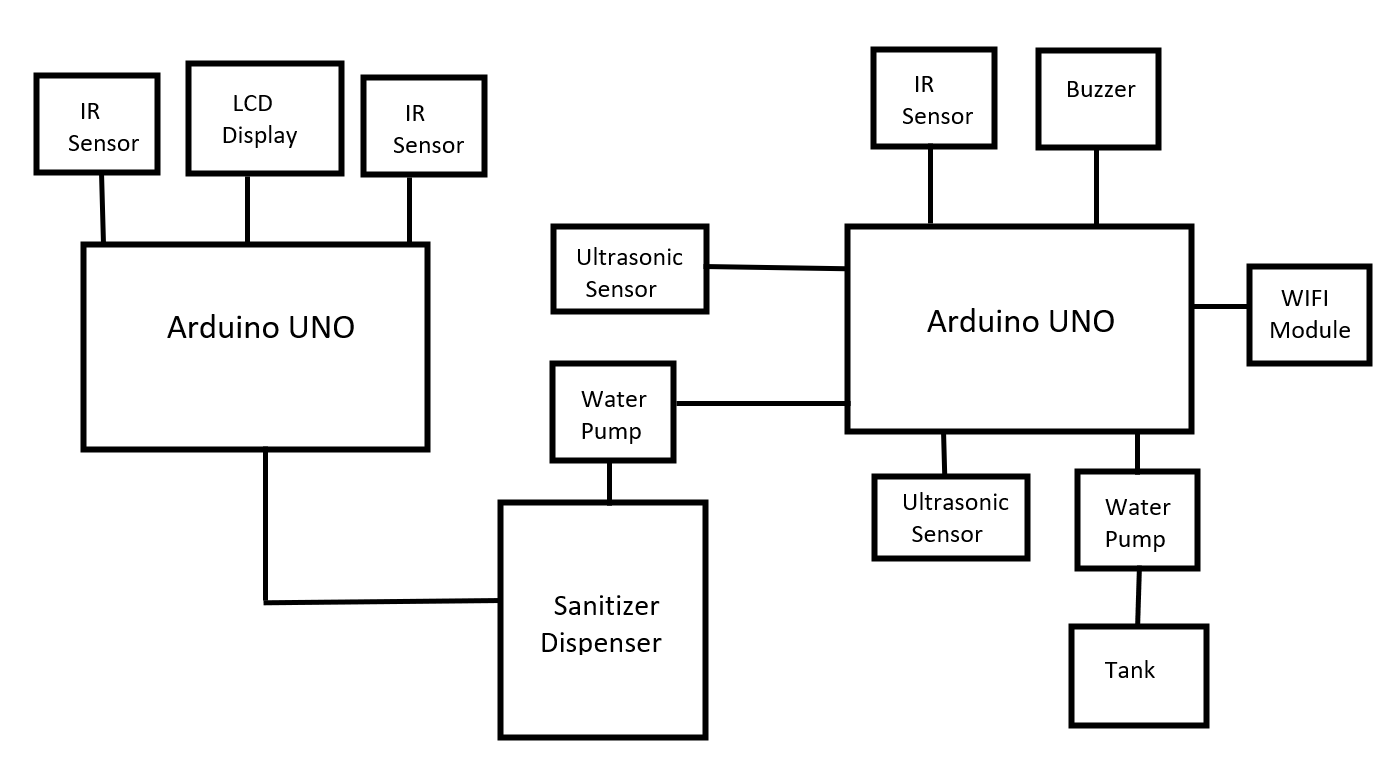
\includegraphics[width=150mm,scale=1]{block}
	\caption{Block Diagram}
	\label{Block Diagram}
	\end{figure}
  \vspace{0.5cm}
  
  \hspace{0.5cm} In this project we have used two Arduinos. One is for Bidirectional visitor counter and other for dispenser and automatic tank filling system. At first Arduino 2 IR sensors are connected for counting number of people entering and leaving premises. At same LCD is connected for display counting. At second Arduino 2 water pumps and 2 ultrasonic sensors are connected. One is for dispense sanitizer liquid and another is for automatic sanitizer tank filling. At this Arduino IR sensor and Buzzer is connected for alert system and WIFI module is connected for sending Alert SMS.

  
 



%% refer q31.tex
%% include the topic name as per u r project in appendix
\chapter{Design and Implementation}

\section{Hardware}
\subsection{Arduino UNO}
 
	\begin{figure}[h]
		\centering
	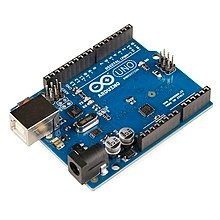
\includegraphics[width=60mm,scale=1]{41}
	\caption{Arduino Uno}
	\label{Arduino}
	
\end{figure}
 
 Arduino is an open-source platform used for building electronics projects. Arduino consists of both a physical programmable circuit board (often referred to as a microcontroller) and a piece of software, or IDE (Integrated Development Environment) that runs on your computer, used to write and upload computer code to the physical board. The Arduino platform has become quite popular with people just starting out with electronics, and for good reason. Unlike most previous programmable circuit boards, the Arduino does not need a separate piece of hardware (called a programmer) in order to load new code onto the board you can simply use a USB cable. Additionally, the Arduino IDE uses a simplified version of C++, making it easier to learn to program. Arduino uno has 14 digital input/output pins (of which 6 can be used as PWM outputs), 6 analog inputs, a USB connection, a power jack, a reset button and more. It contains everything needed to support the microcontroller; simply connect it to a computer with a USB cable or power it with a AC-to-DC adapter or battery.
 
 Arduino was born at the Ivrea Interaction Design Institute as an easy tool for fast prototyping, aimed at students without a background in electronics and programming. As soon as it reached a wider community, the Arduino board started changing to adapt to new needs and challenges, differentiating its offer from simple 8-bit boards to products for IoT applications, wearable, 3D printing, and embedded environments. All Arduino boards are completely open-source, empowering users to build them independently and eventually adapt them to their particular needs. The software, too, is open-source, and it is growing through the contributions of users worldwide.
 
 
\newpage
\subsection{Bolt WIFI Module} 

	\begin{figure}[h]
		\centering
	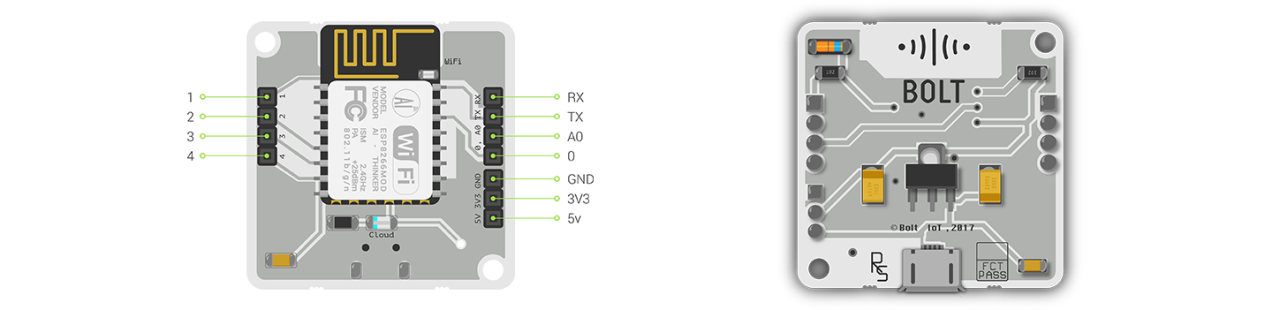
\includegraphics[width=120mm,scale=1]{42}
	\caption{Bolt WIFI Module}
	\label{Bolt WIFI Module}
	
\end{figure}

 The bolt Wifi module contains ESP8266 Wifi module. The ESP8266 Wifi Module is a self-contained SOC with integrated TCP/IP protocol stack that can give any microcontroller access to your Wifi network. The ESP8266 is capable of either hosting an application or offloading all Wi-Fi networking functions from another application processor. The ESP8266 module is an extremely cost effective board. 
 
 This module has a powerful enough on-board processing and storage capability that allows it to be integrated with the sensors and other application specific devices through its GPIOs with minimal development up-front and minimal loading during runtime. Its high degree of on-chip integration allows for minimal external circuitry, including the front-end module, is designed to occupy minimal PCB area.
 
\newpage
\subsection{HC-SR04 Ultrasonic Sensor}
 
	\begin{figure}[h]
		\centering
	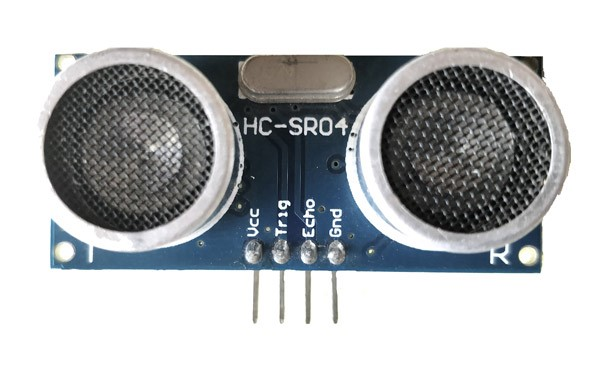
\includegraphics[width=60mm,scale=1]{43}
	\caption{HC-SR04 Ultrasonic Sensor}
	\label{HC-SR04 Ultrasonic Sensor}
	
\end{figure}

 The HC-SR04 ultrasonic sensor uses SONAR to determine the distance of an object just like the bats do. It offers excellent non-contact range detection with high accuracy and stable readings in an easy-to-use package from 2 cm to 400 cm or 1” to 13 feet.  It comes complete with ultrasonic transmitter and receiver module. Operating voltage: +5V  Theoretical Measuring Distance: 2cm to 450cm. Practical Measuring Distance: 2cm to 80cm.
 
  Power the Sensor using a regulated +5V through the Vcc ad Ground pins of the sensor. The current consumed by the sensor is less than 15mA and hence can be directly powered by the on board 5V pins (If available). The Trigger and the Echo pins are both I/O pins and hence they can be connected to I/O pins of the microcontroller. To start the measurement, the trigger pin has to be made high for 10uS and then turned off. This action will trigger an ultrasonic wave at frequency of 40Hz from the transmitter and the receiver will wait for the wave to return. Once the wave is returned after it getting reflected by any object the Echo pin goes high for a particular amount of time which will be equal to the time taken for the wave to return back to the sensor.
 
\newpage

\subsection{IR Sensor}

	\begin{figure}[h]
		\centering
	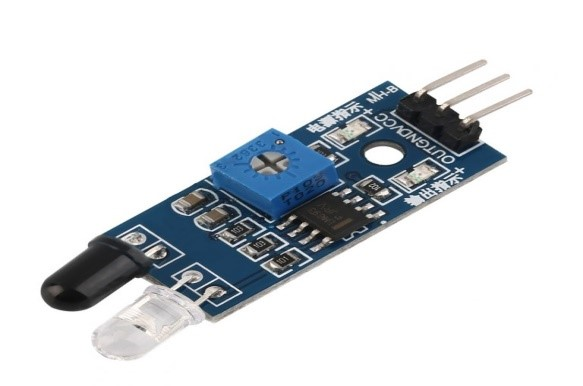
\includegraphics[width=60mm,scale=1]{44}
	\caption{IR Sensor}
	\label{IR Sensor}
	
\end{figure}

 IR sensor is an electronic device, that emits the light in order to sense some object of the surroundings. An IR sensor can measure the heat of an object as well as detects the motion. Usually, in the infrared spectrum, all the objects radiate some form of thermal radiation. These types of radiations are invisible to our eyes, but infrared sensor can detect these radiations.
 
  The emitter is simply an IR LED (Light Emitting Diode) and the detector is simply an IR photodiode . Photodiode is sensitive to IR light of the same wavelength which is emitted by the IR LED. When IR light falls on the photodiode, the resistances and the output voltages will change in proportion to the magnitude of the IR light received.
 
\newpage 
\subsection{Buzzer}

	\begin{figure}[h]
		\centering
	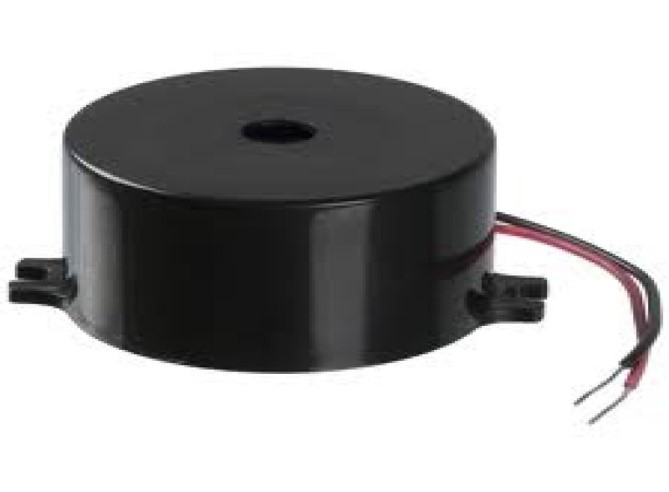
\includegraphics[width=60mm,scale=1]{45}
	\caption{Buzzer}
	\label{Buzzer}
	
\end{figure}

 A buzzer or beeper is an audio signalling device, which may be mechanical,electromechanical, or piezoelectric (piezo for short). Typical uses of buzzers and beepers include alarm devices, timers, of user input such as a mouse click or keystroke.
 
 The buzzer consists of an outside case with two pins to attach it to power and ground. Inside is a piezo element, which consists of a central ceramic disc surrounded by a metal (often bronze)vibration disc. When current is applied to the buzzer it causes the ceramic disk to contract or expand.A buzzer converts
electricity into sound when current flows through it. It is drawn as half a circle with two short lines extending down.  
 
\newpage

\subsection{LCD Display}

	\begin{figure}[h]
		\centering
	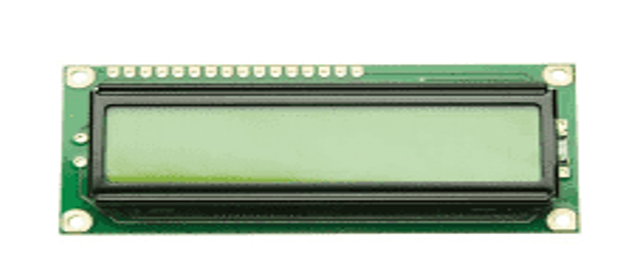
\includegraphics[width=60mm,scale=1]{46}
	\caption{LCD Display}
	\label{LCD Display}
	
\end{figure}

 LCD (Liquid Crystal Display) is a type of at panel display which uses liquid crystals in its primary form of operation. LEDs have a large and varying set of use cases for consumers and businesses, as they can be commonly found in smartphones, televisions, computer monitors and instrument panels. Liquid crystal display technology works by blocking light.
  
 At the same time, electrical currents cause the liquid crystal molecules to align to allow varying levels of light to pass through to the second substrate and create the colors and images that you see.Since LCD screens do not use phosphors, they rarely suffer image burn-in when a static image is displayed on a screen for a long time, e.g, the table frame for an airline light schedule on an indoor sign. LCDs are, however, susceptible to image persistence.The LCD screen is more energy-efficient and can be disposed of more safely than a CRT can. Its low electrical power consumption.
 
\newpage

\subsection{Mini Pump}

	\begin{figure}[h]
		\centering
	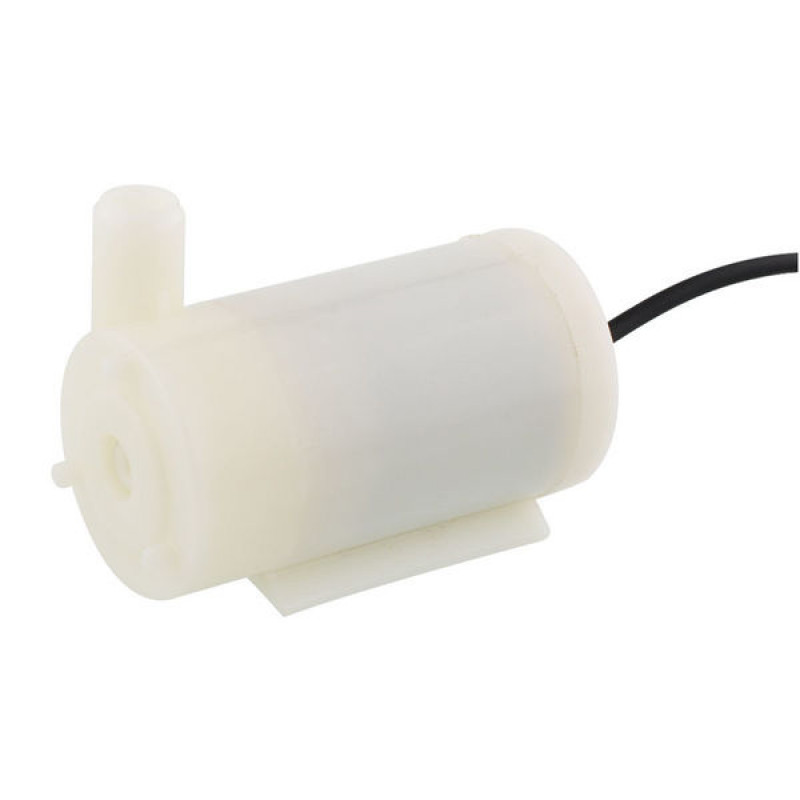
\includegraphics[width=60mm,scale=1]{47}
	\caption{Mini Pump}
	\label{Mini Pump}
	
\end{figure}
Submersible pumps in general are designed to be fully submerged into the water. Submersible pumps are placed within the reservoir of water that requires pumping out, which is why they are normally used for drainage in floods, sewerage pumping, emptying ponds or even as pond filters.

A mini submersible water pump is a centrifugal water pump, which means that it uses a motor to power an impeller that is designed to rotate and push water outwards. The motor is located in a waterproof seal and closely connected to the body of the water pump which it powers.

Mini water motor pump is mini type to transfer sanitizer from lower place to higher place or too far place.It is used in refilling system to Refill the sanitizer bottle.

\newpage

\subsection{L293D MOTOR DRIVER IC}

	\begin{figure}[h]
		\centering
	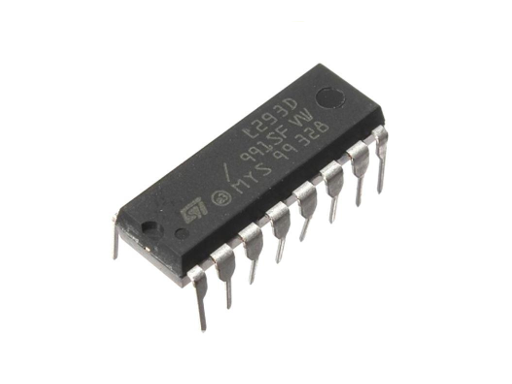
\includegraphics[width=60mm,scale=1]{48}
	\caption{L293D MOTOR DRIVER IC}
	\label{L293D MOTOR DRIVER IC}
	
\end{figure}

L293D is a typical Motor driver or Motor Driver IC which allows DC motor to drive on either direction. L293D is a 16-pin IC which can control a set of two DC motors simultaneously in any direction. It means that you can control two DC motor with a single L293D IC.The l293d can drive small and quiet big motors as well.

It works on the concept of H-bridge. H-bridge is a circuit which allows the voltage to be flown in either direction. As you know voltage need to change its direction for being able to rotate the motor in clockwise or anticlockwise direction, Hence H-bridge IC are ideal for driving a DC motor.In a single L293D chip there are two h-Bridge circuit inside the IC which can rotate two dc motor independently. Due its size it is very much used in robotic application for controlling DC motors.

\newpage

\section{Software}
\subsection{Ardiuno IDE}

\begin{figure}[h]
		\centering
	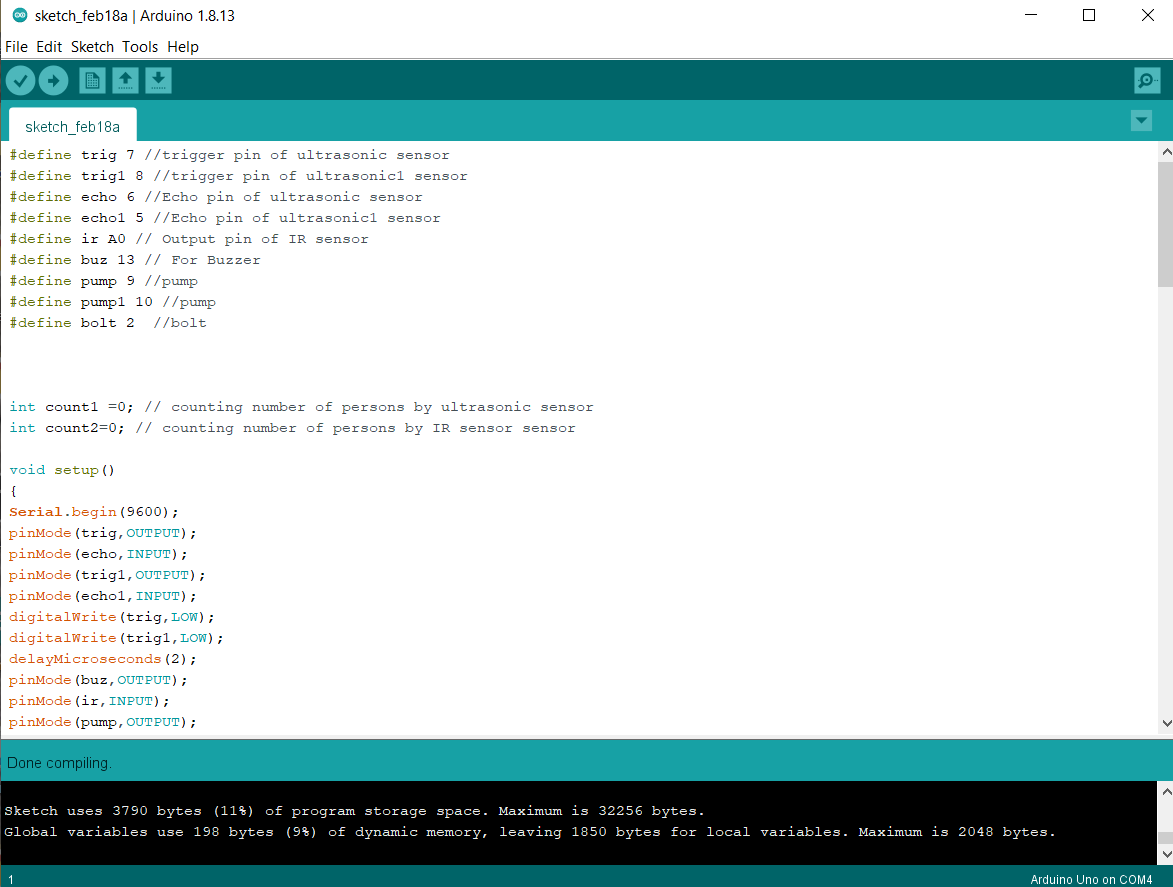
\includegraphics[width=120mm,scale=1]{49}
	\caption{Ardiuno IDE}
	\label{Ardiuno IDE}
	
\end{figure}

The Arduino Integrated Development Environment (IDE) is a cross-platform application (for Windows, macOS, Linux) that is written in functions from C and C++. It is used to write and upload programs to Arduino compatible boards. The Arduino IDE supplies a software library from the Wiring project, which provides
many common input and output procedures. User-written code only requires two basic functions, for starting the sketch and the main program loop, that are compiled and linked with a program stub main() into an executable cyclic executive program with the GNU toolchain, also included with the IDE distribution. Active development of the Arduino software is hosted by GitHub.The open source Arduino IDE editor allows you to write code and easily load it to the controllers via USB. The Arduino IDE supports many different   controllers besides Arduino kits (Uno, Pro Mini, Mega, Due etc.).

This software works on Windows, Mac OS X and Linux. The Arduino IDE is written in the Java language and is based on the language named Processing/Wiring. The libraries are written in C and C ++ languages and compiled with AVR-GCC and AVR Libc. There are many other microcontrollers and microcontroller platforms available for physical computing. Parallax Basic Stamp, Netmedia’s BX-24, Phidgets, MIT’s Handyboard, and many others offer similar functionality. All of these tools take the messy details of microcontroller programming and wrap it up in an easy-to-use package. Arduino also simplifies the process of working with microcontrollers its Simple, clear programming environment and Inexpensive.

\newpage

\subsection{Virtual Box}

\begin{figure}[h]
		\centering
	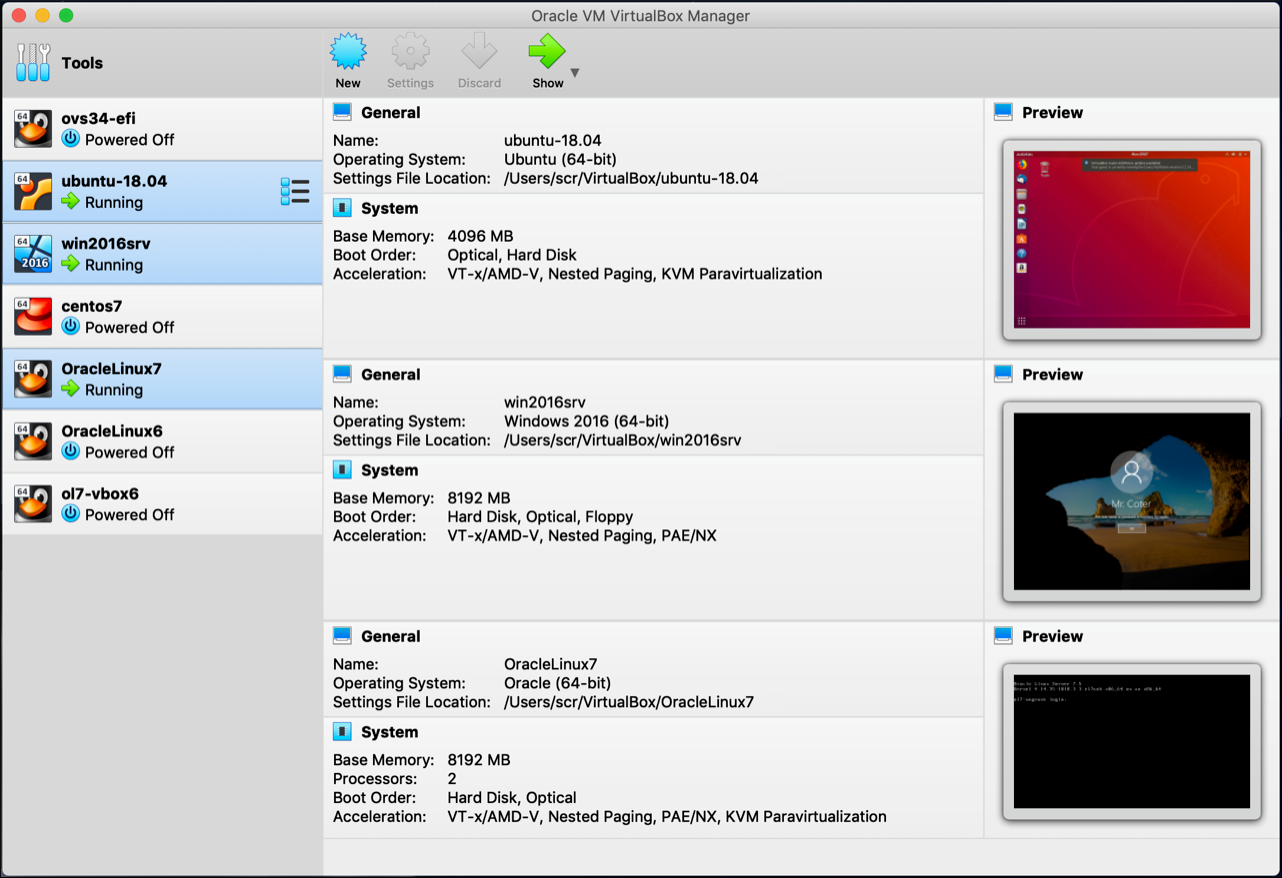
\includegraphics[width=120mm,scale=1]{51}
	\caption{Virtual Box}
	\label{Virtual Box}
	
\end{figure}

Oracle VM VirtualBox is a free and open-source hosted hypervisor for x86 virtualization, developed by Oracle Corporation. Created by Innotek, it was acquired by Sun Microsystems in 2008, which was in turn acquired by Oracle in 2010. VirtualBox may be installed on Windows, macOS, Linux, Solaris and OpenSolaris. There are also ports to FreeBSD and Genode. It supports the creation and management of guest virtual machines running Windows, Linux, BSD, OS/2, Solaris, Haiku, and OSx86,as well as limited virtualization of macOS guests on Apple hardware. For some guest operating systems, a "Guest Additions" package of device drivers and system applications is available,which typically improves performance, especially that of graphics.

\newpage

\subsection{Twilio}



\hspace{0.5cm} Twilio is a third-party SMS functionality provider. It is a cloud communications platform as a service (PaaS) company. Twilio allows software developers to programmatically make and receive phone calls and also send and receive text messages using its web service APIs.

\vspace{0.4cm}

\begin{figure}[h]
		\centering
	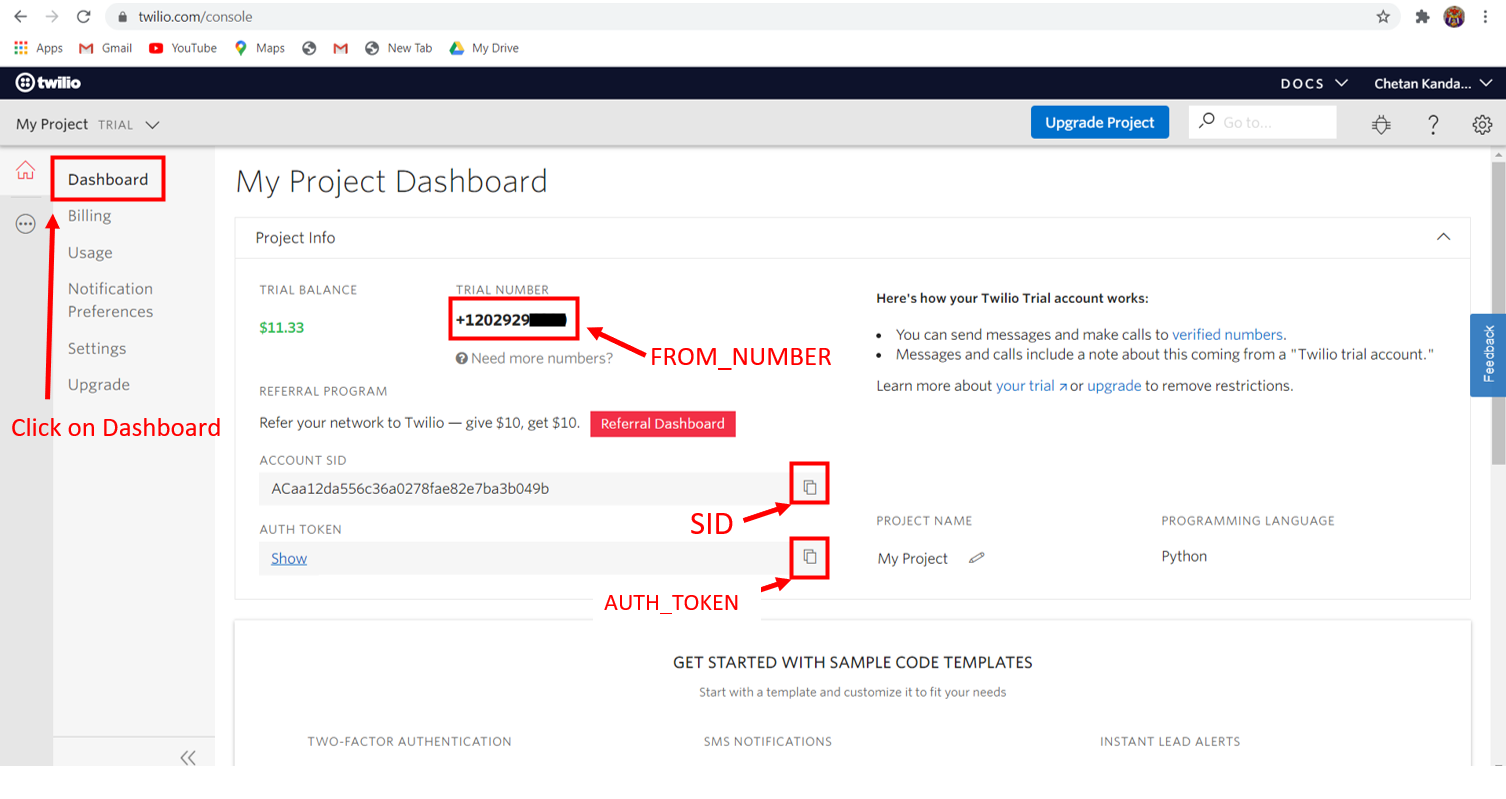
\includegraphics[width=120mm,scale=1]{50}
	\caption{Twilio}
	\label{Twilio}
	
\end{figure}

Creating an account on Twilio

\vspace{0.4cm}

Step 1: Open https://www.twilio.com/  in browser.
\vspace{0.4cm}

Step 2: Click on  Get a Free API Key button to sign up.

\vspace{0.4cm}
Step 3: Fill all the necessary details in SIGN UP form.

\vspace{0.4cm}
Step 4: To verify they will ask for your phone number. Choose India as an option in the dropdown and then enter your phone number.

\vspace{0.4cm}
Step 5: Click on "Products". Now enable the SMS services by clicking on two checkboxes for Programmable SMS and Phone Numbers. Once you have done this, scroll to the bottom of the screen and click on "Continue".

\vspace{0.4cm}
Step 6: Now, you will need to give a name for your project. I have given the name as My Project. Click on "Continue" once you have entered the project name.

\vspace{0.4cm}
Step 7: Click on "Skip this step" when it asks you to Invite a Teammate.

\vspace{0.4cm}
Step 8: Your project should be created at this point. Click on "Project Info" to view the account credentials which is required for your projects.

\vspace{0.4cm}
Step 9: You can view the Account SID and Auth token on this page. The Auth token is not visible by   default, you can click on "view" button to make the Auth token visible.

\vspace{0.4cm}
Step 10: From the drop-down menu, choose "Programmable SMS". Now click on Get Started button to generate  phone number.

\vspace{0.4cm}
Step 11: Click on Get a number button.

\vspace{0.4cm}
Step 12: Then a popup will appear. Click on Choose this number button.

\vspace{0.4cm}
Step 13: Then a popup will appear which will have the final number.


\vspace{0.5cm}
Copy the SID, AUTH TOKEN, FROM NUMBER for entering in the python code.


\vspace{0.4cm}
Install Ubuntu on Virtual Box.

Go to your ubuntu terminal and install the required software using the following instructions.

\vspace{0.2cm}

\textbf{sudo apt-get -y update}

\textbf{sudo apt install python3-pip}

\textbf{sudo pip3 install boltiot}

\vspace{0.5cm}



\newpage

\section{Flow Chart}

\begin{figure}[h]
		\centering
	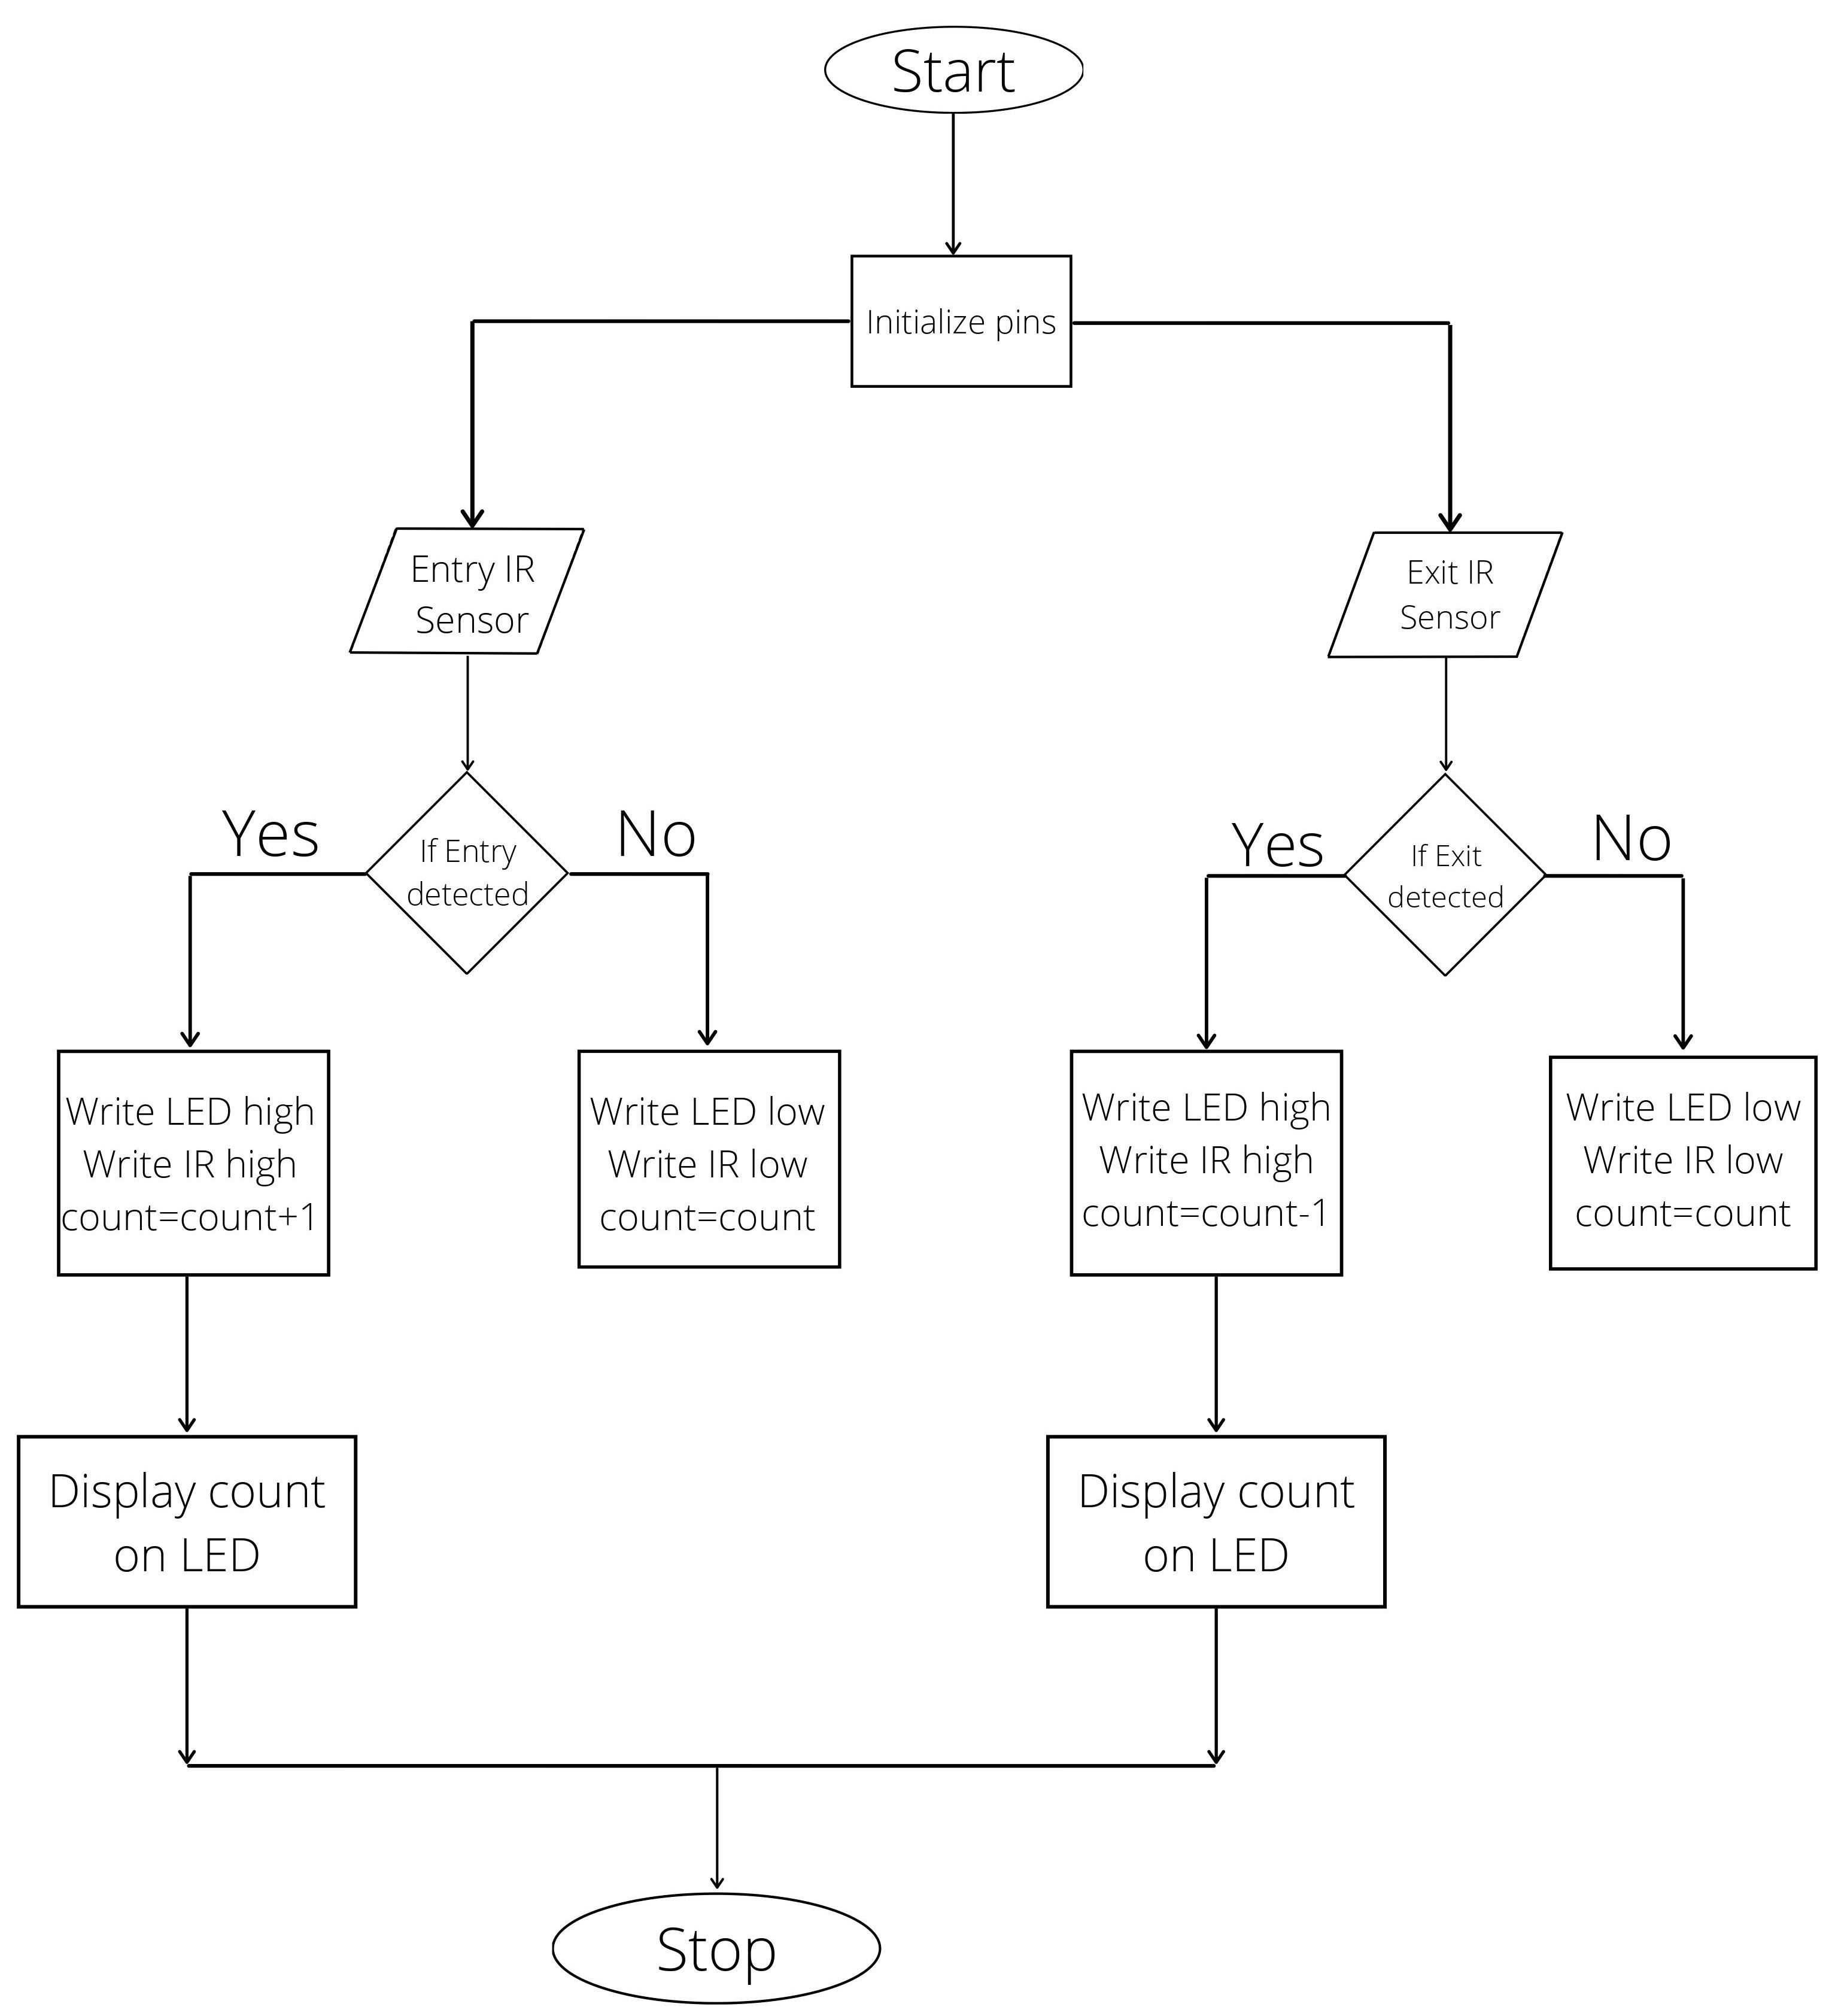
\includegraphics[width=135mm,scale=1]{flowchart1}
	\caption{Bidirectional Visitor Couter Flow Chart}
	\label{Bidirectional Visitor Couter Flow Chart}
	
\end{figure}

\begin{figure}[h]
		\centering
	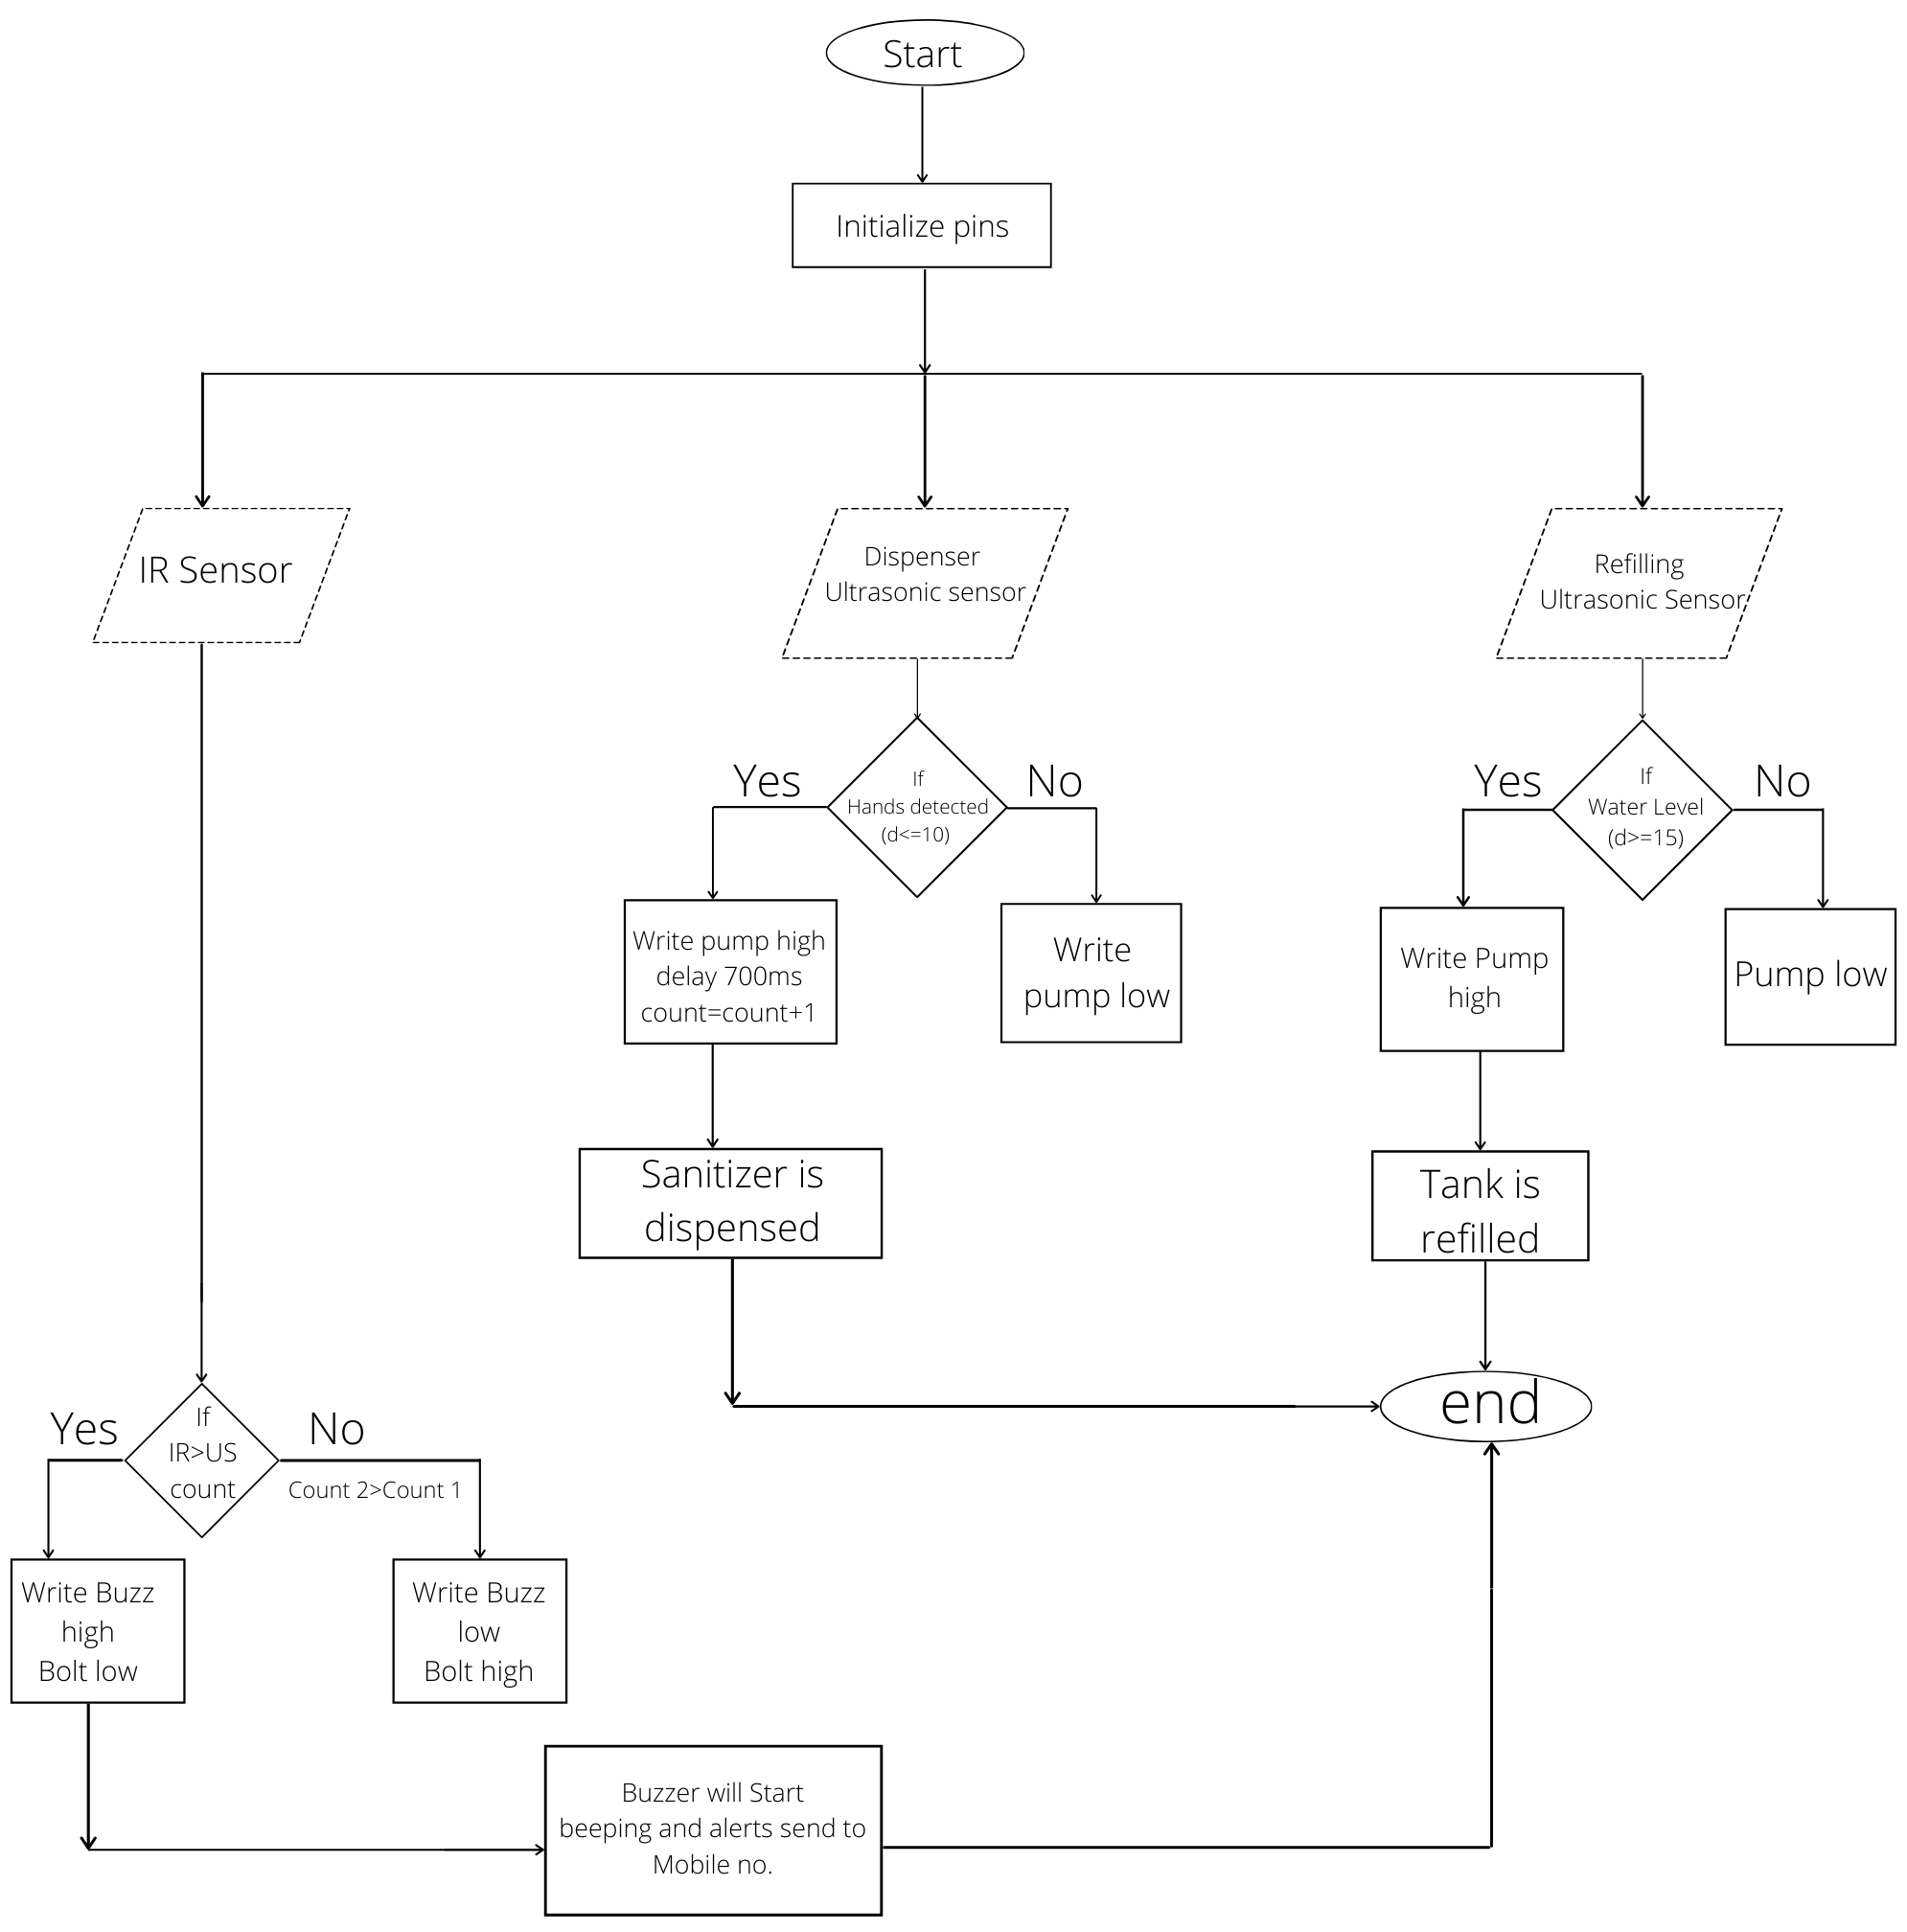
\includegraphics[width=150mm,scale=1]{flowchart2}
	\caption{Dispenser and Autofilling tank system Flow Chart}
	\label{Dispenser and Autofilling tank system Flow Chart}
	
\end{figure}








\chapter{Hardware Implementation}


\section{Bidirectional Visitor Counter}

   \begin{figure}[h]
		\centering
	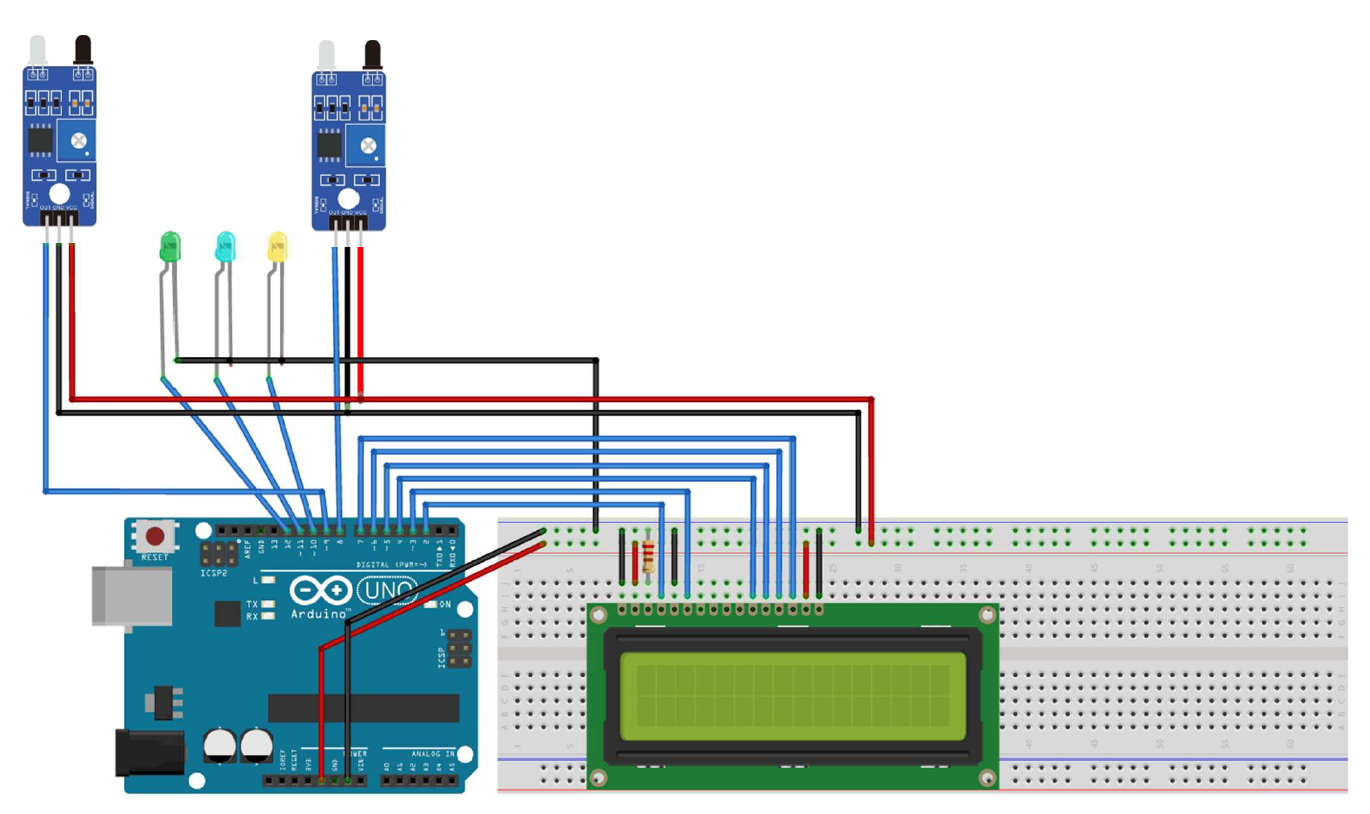
\includegraphics[width=140mm,scale=1]{circuit1}
	\caption{Circuit Connection 1}
	\label{Bidirectional Visitor Counter}
\end{figure}


\newpage
\section{Dispenser and Automatic tank filling system}

   \begin{figure}[h]
		\centering
	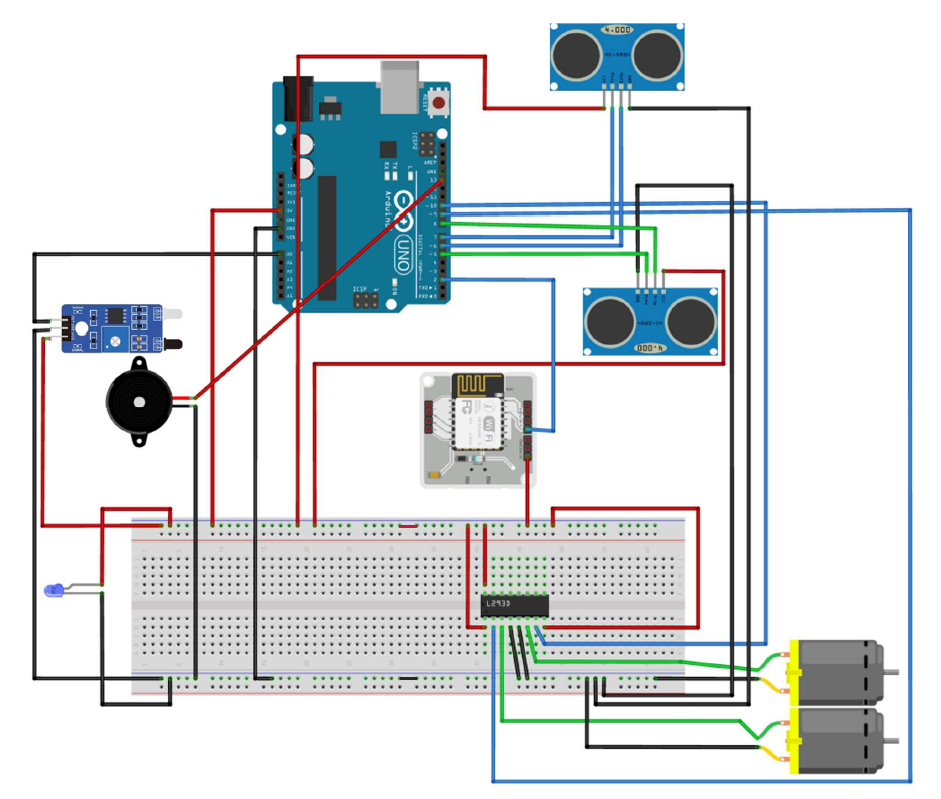
\includegraphics[width=140mm,scale=1]{circuit2}
	\caption{Circuit Connection 2}
	\label{Bidirectional Visitor Counter}
\end{figure}
\newpage
\thispagestyle{empty}

\chapter{Results}

	\hspace{0.5cm} We've built an IoT-based automatic hand sanitizer dispenser with features including automatic refilling, hand sanitizer alerts, visitor counters and automatic dispensing.
	In the first step, we created a hand sanitizer dispenser with an    ultrasonic sensor that detects the user's hand. Sanitizer is dispensed as soon as hands are sensed. We created an alert system in which if anyone attempts to access the premises without sanitising their hands, a buzzer would beep continuously.Simultaneously, an alert SMS is sent to the registered mobile number. 
	After that, we built a bidirectional visitor counter to keep track of the number of persons entering and exiting the building, or in other words, the number of people present inside the building. We created an automated sanitizer refilling device at the end of the project. This feature automatically refills the sanitizer bottle when it reaches a certain level.
	
\newpage

	\begin{figure}[h]
		\centering
	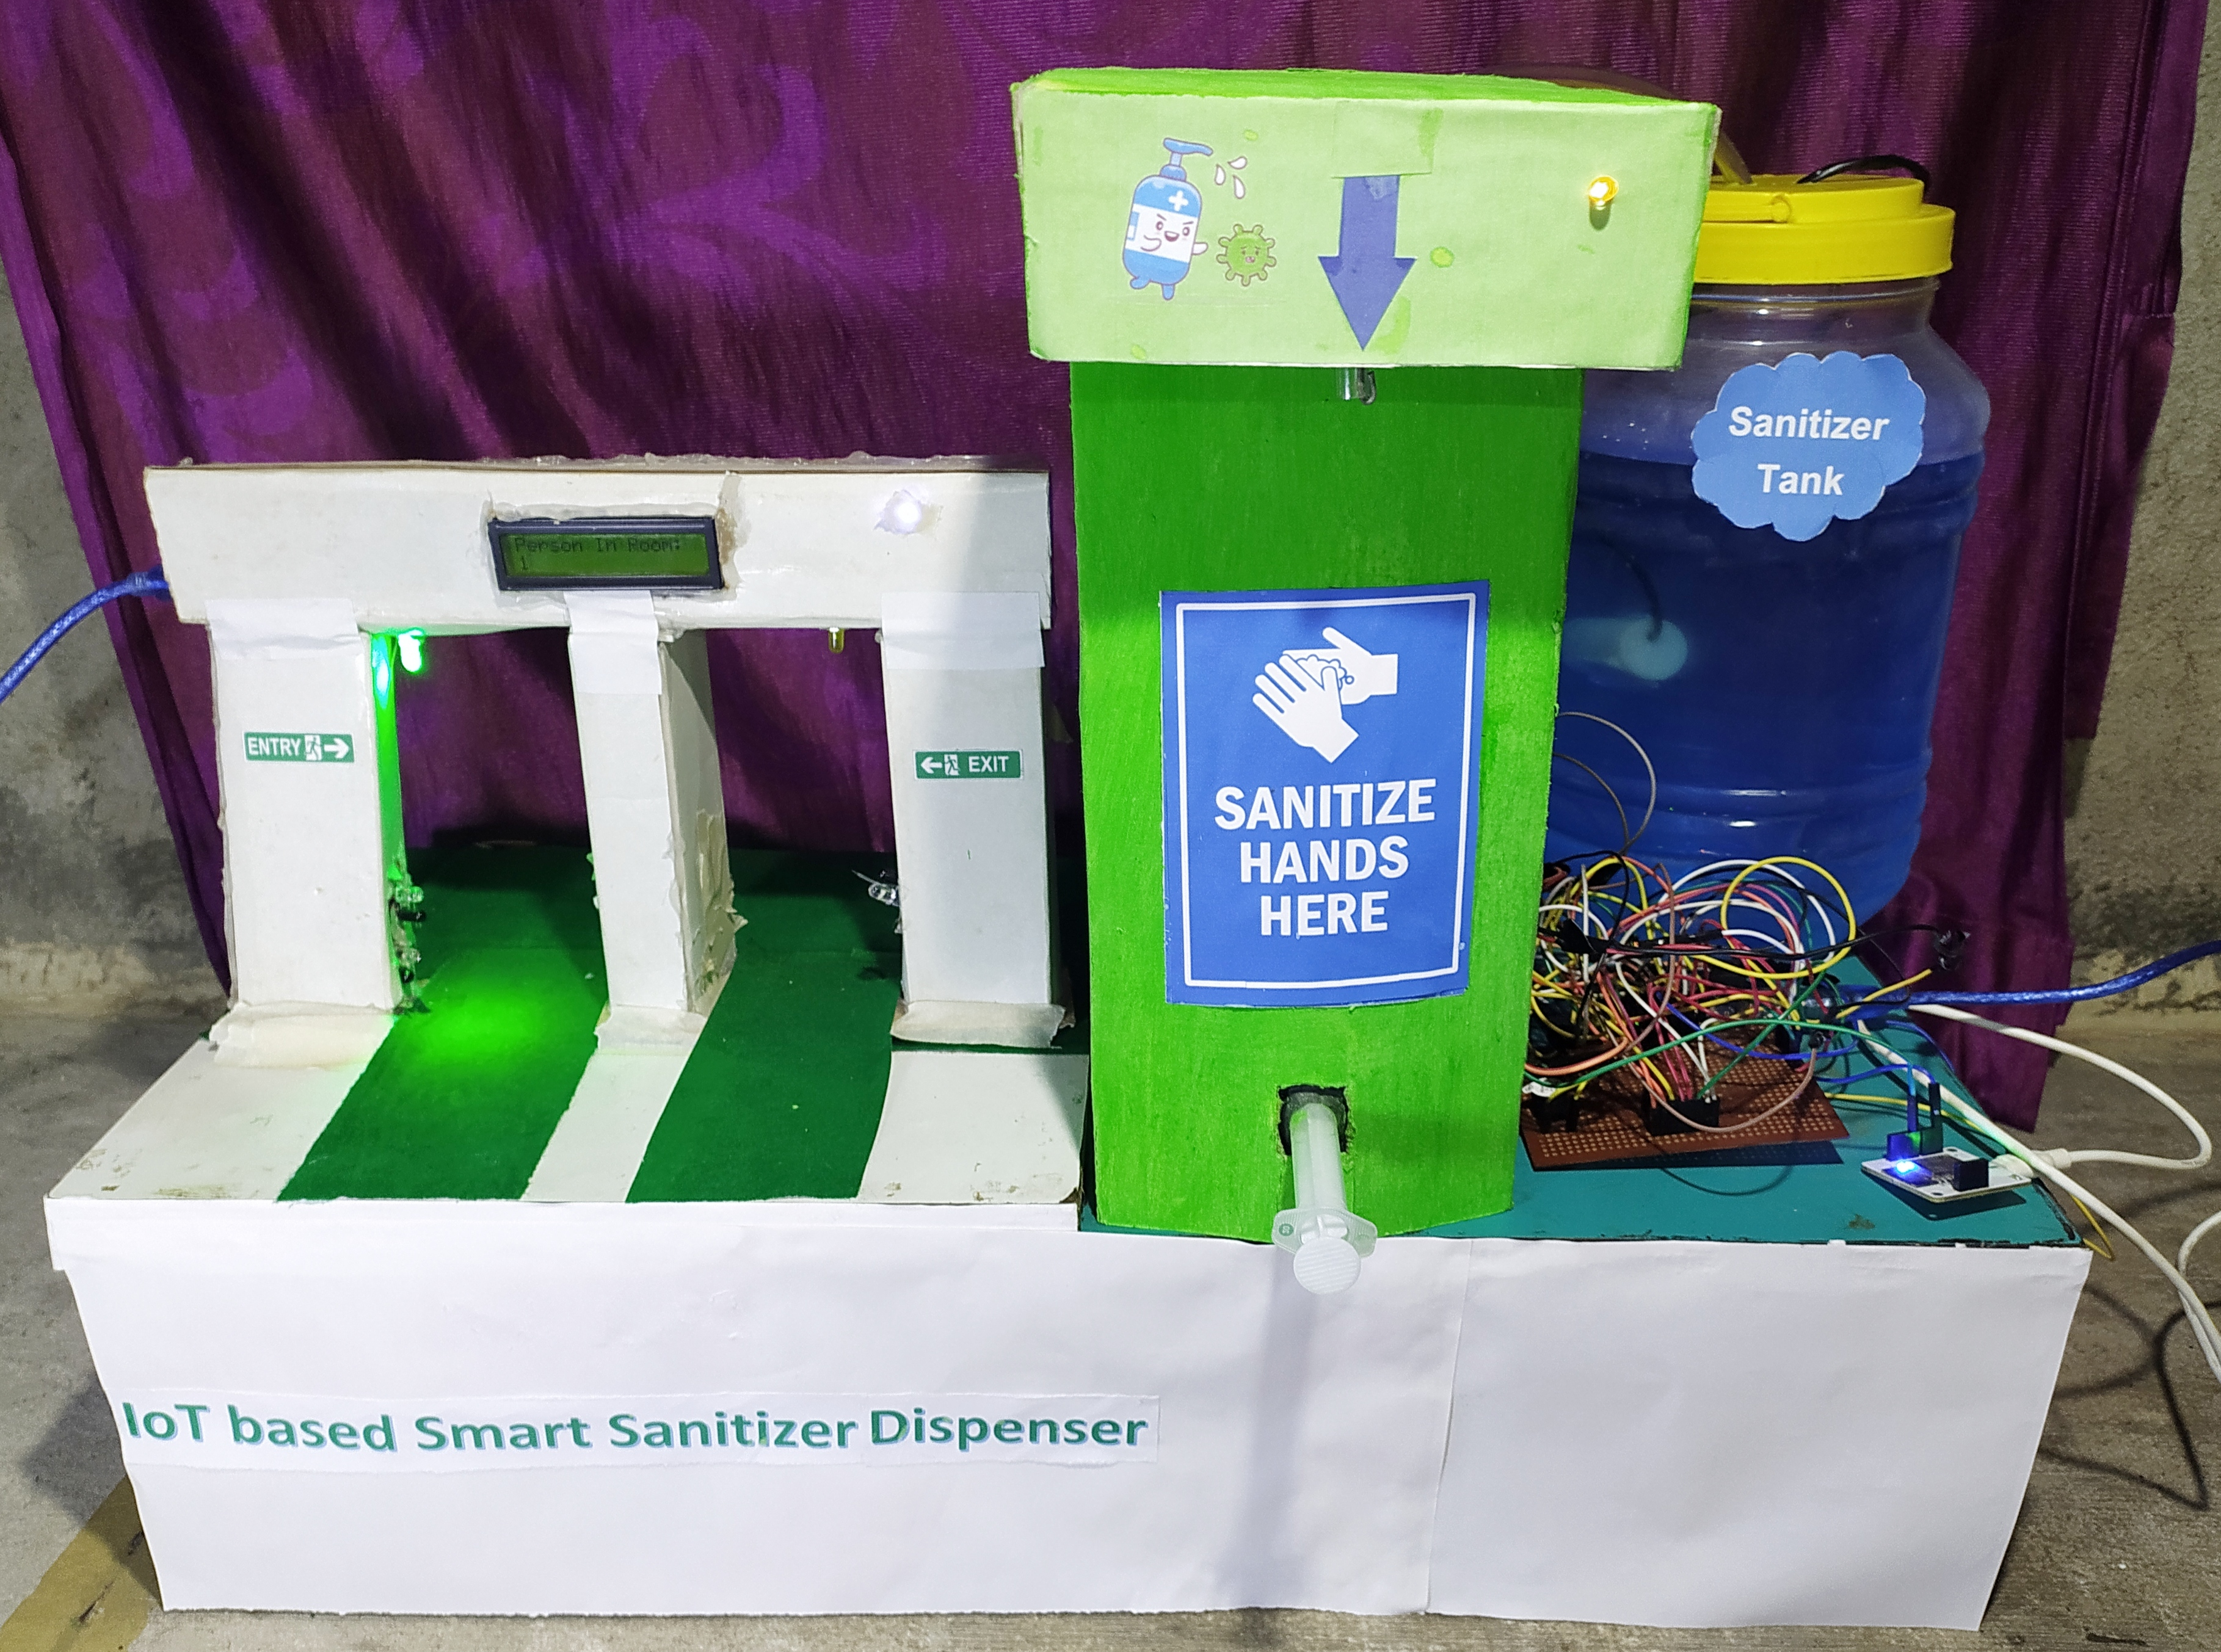
\includegraphics[width=80mm,scale=1]{result1}
	\caption{Project Model}
	\label{Project Model}
	
\end{figure}

\vspace{1cm}
	\begin{figure}[h]
		\centering
	\includegraphics[width=45mm,scale=1]{result2}
	\caption{Sanitizer Dispenser}
	\label{Sanitizer Dispenser}
	
\end{figure}

\newpage

	\begin{figure}[h]
		\centering
	\includegraphics[width=75mm,scale=1]{result3}
	\caption{Bidirectional Visitor Counter}
	\label{Bidirectional Visitor Counter}
	
\end{figure}

\vspace{1cm}
	\begin{figure}[h]
		\centering
	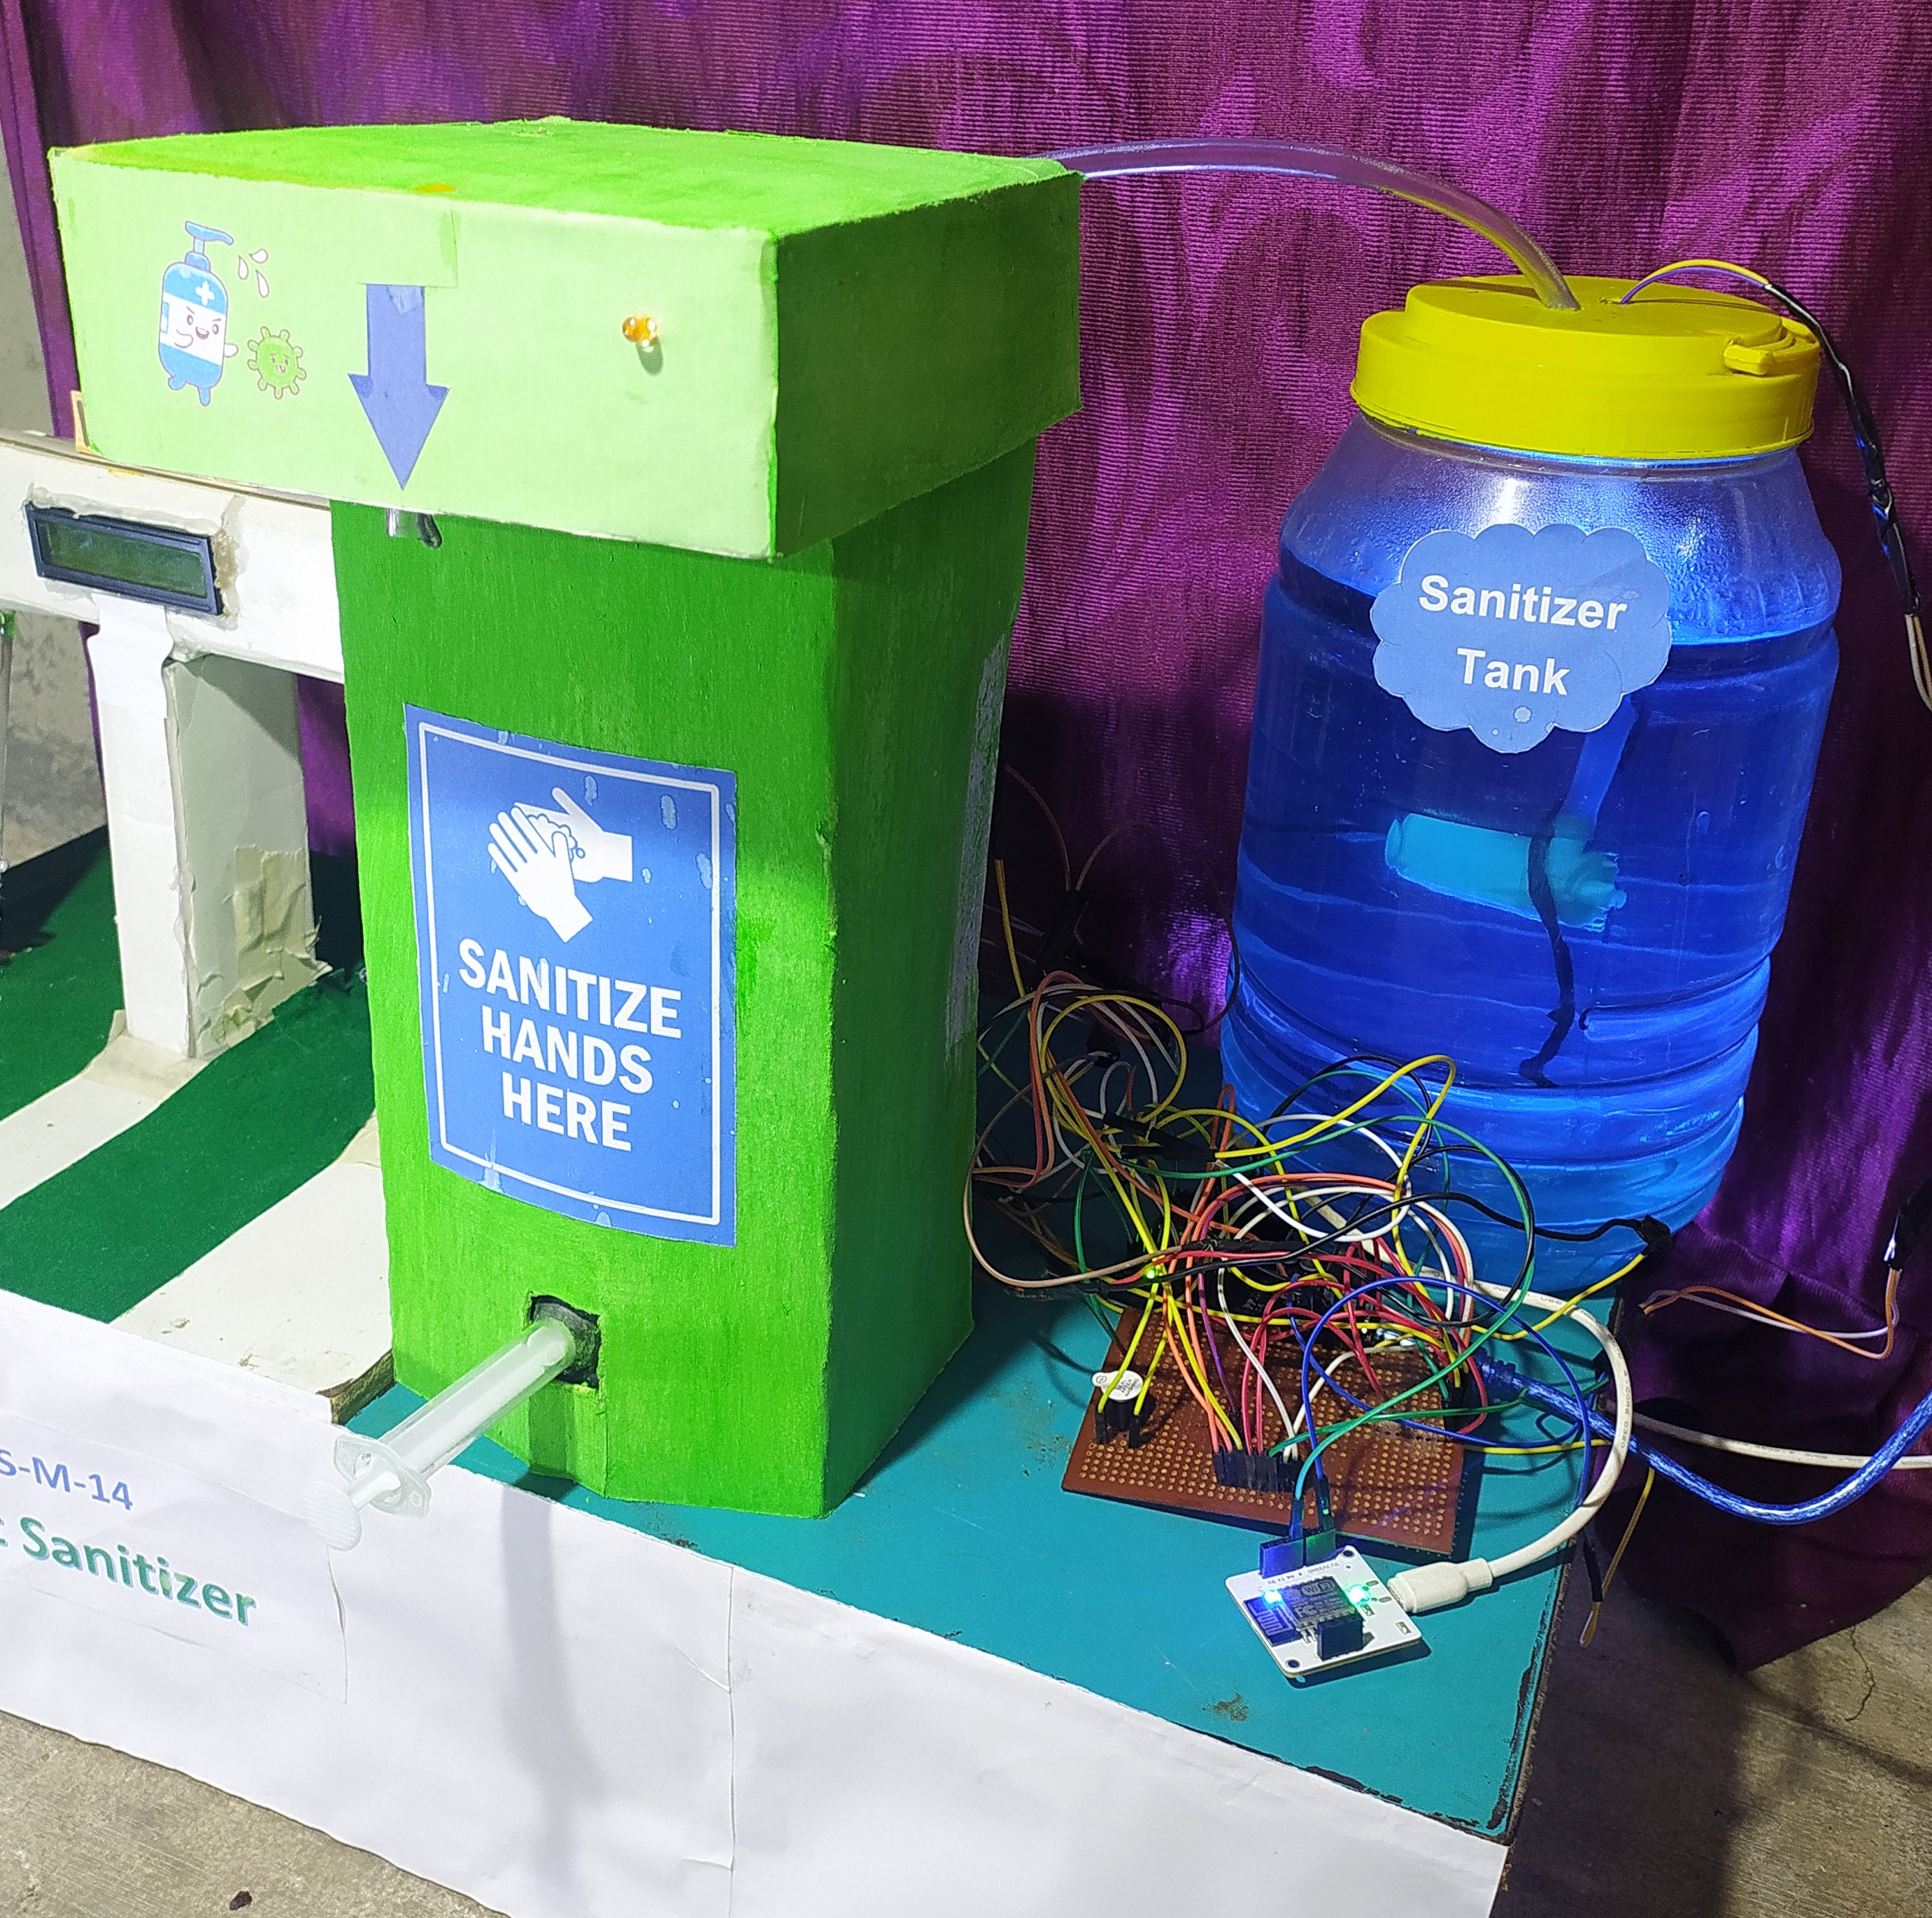
\includegraphics[width=75mm,scale=1]{result4}
	\caption{Automatic tank filling system}
	\label{Automatic tank filling system}
	
\end{figure}

\newpage

	\begin{figure}[h]
		\centering
	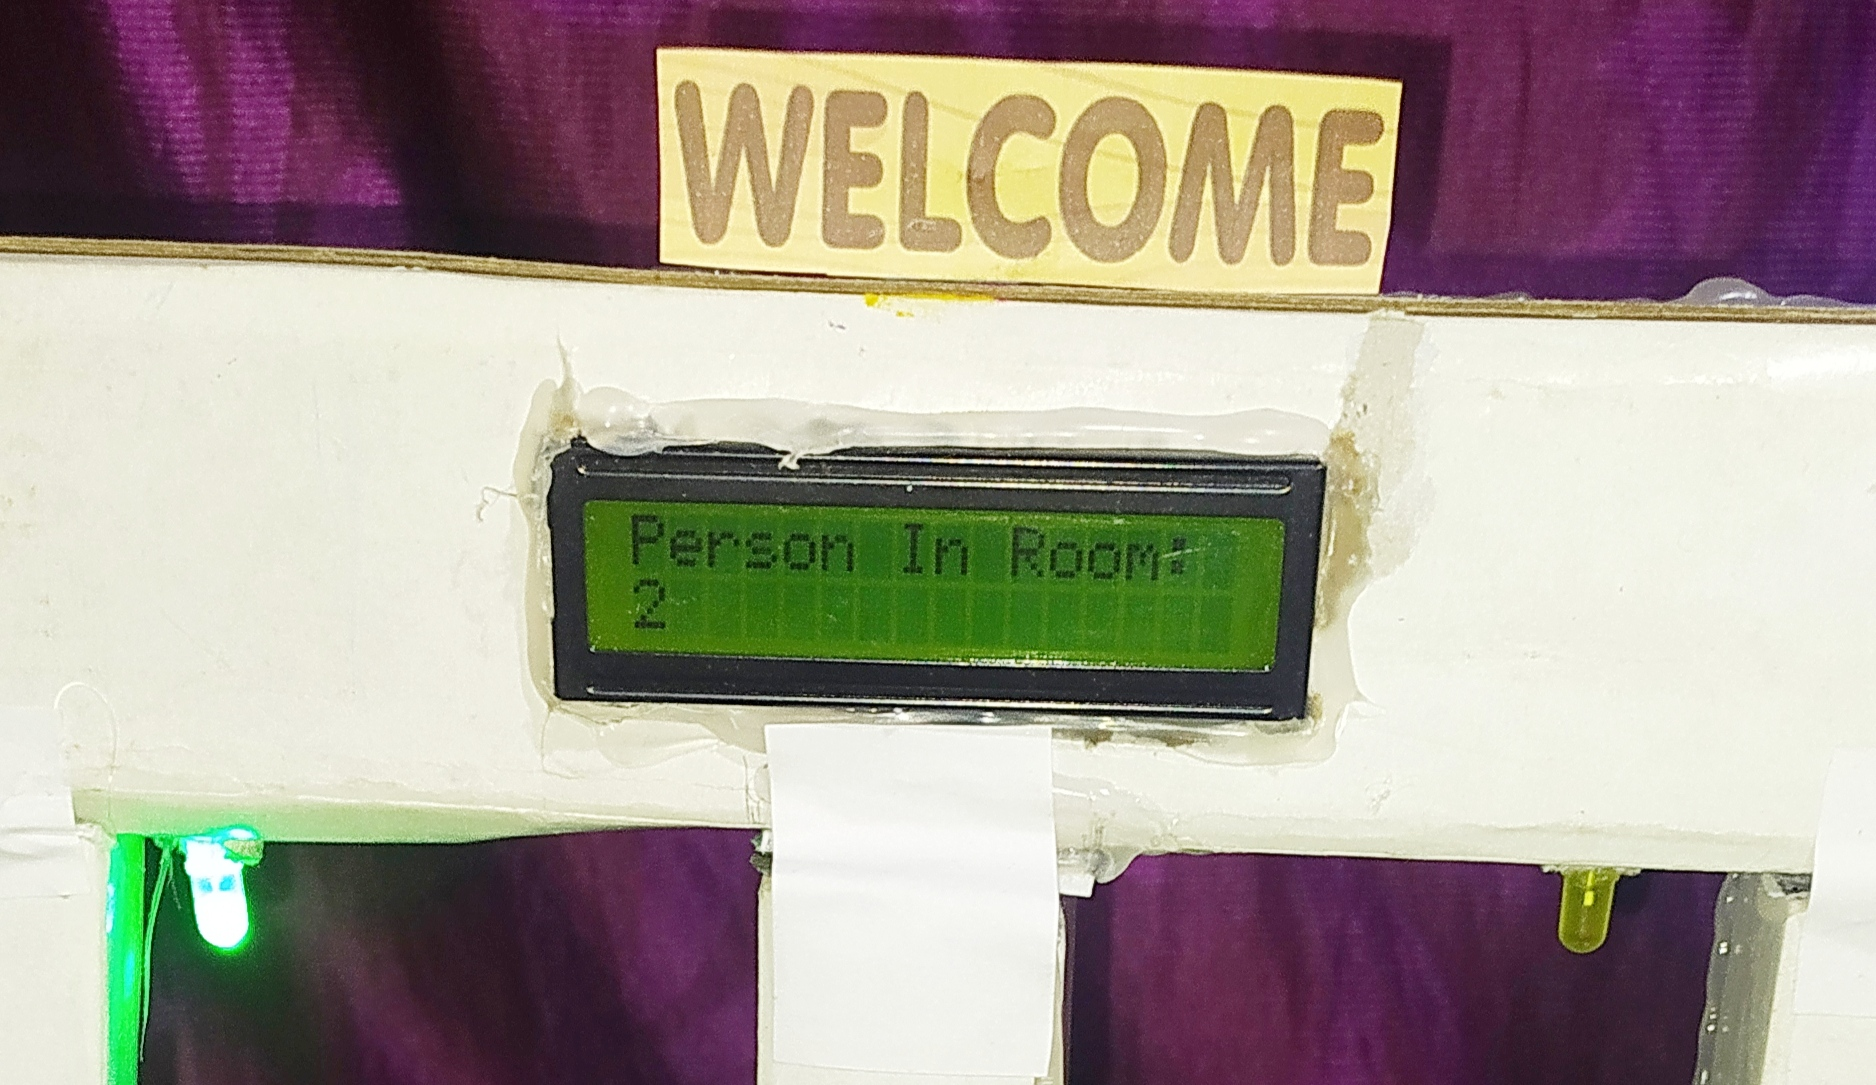
\includegraphics[width=80mm,scale=1]{result5}
	\caption{Visitor Counter Display}
	\label{Visitor Counter Display}
	
\end{figure}

\vspace{1cm}
	\begin{figure}[h]
		\centering
	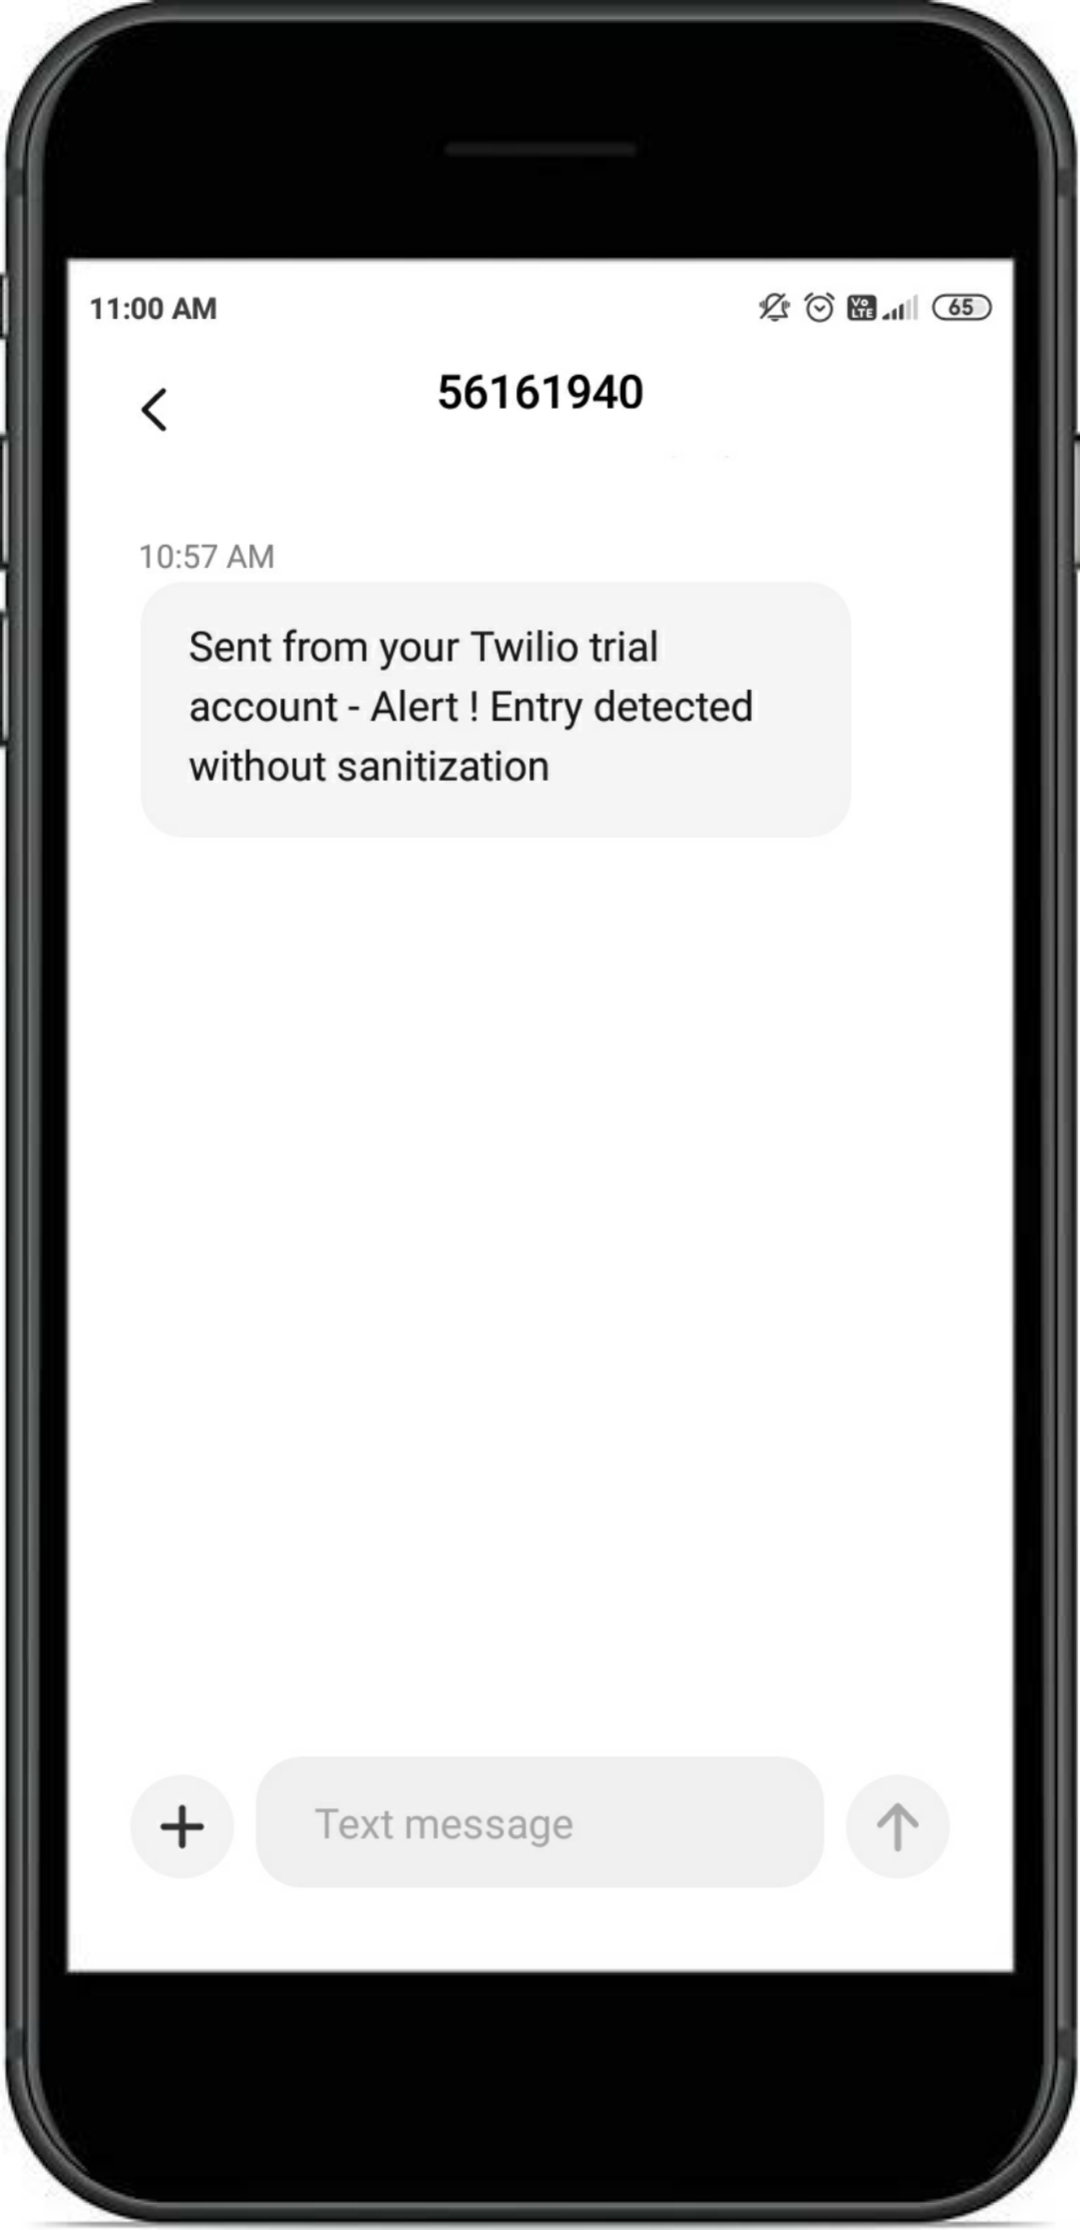
\includegraphics[width=41mm,scale=1]{result6}
	\caption{Alert SMS}
	\label{Alert SMS}
	
\end{figure}


\newpage
\thispagestyle{empty}

\chapter{Conclusions}

\section{Conclusions}

 \hspace{0.5cm} This project will make smart touchless hand sanitizer system with auto refilling feature to reduce human labour and also possess alarm to remind person to sanitize hand before entering the premises. It also keeps count of persons to monitor the no of persons present in the premises. In current Circumstances, social distancing and constant disinfection of Public places become a necessity. So this Project will be very useful to use in hospitals, bank, mall and many public places.

\newpage
\section{Scope for improvement }
\vspace{1cm} 

  \hspace{0.5cm} In the future, we can install a camera to recognise those who are permitted to enter. Keep an eye on whether people are abiding to social distancing or not. It would also assist in maintaining accurate records. To detect the body temperature, a temperature sensor could be added.We can also add a sms alert system to the sanitizer storage container to send an alert sms when the sanitizer level is low.
\newpage
\thispagestyle{empty}

\chapter{References}

\begin{itemize}
	\item { “The Internet of Things” by Samuel Greengard A guided tour through the Internet of Things, a networked world of connected devices, objects, and people that is changing the way we live and work. 20 March 2015.}
	\item { "Internet of Things: With Arduino and Bolt" By Ashwin Pajankar, India 2018.}
	\item { Bloomfield SF, Aiello AE, Cookson B, O’Boyle C, Larson EL. The effectiveness of hand hygiene procedures in reducing the risks of infections in home and community settings including hand washing and alcohol-based hand sanitizers. Am J Infect Control. 2007}
	\item { Arduino [Internet] Somerville (MA): Arduino; c2020. [cited at 2020 Aug 4]. Available from: https://www.arduino.cc/ [Google Scholar].}
	\item { N. Kaur and S. K. Sood, ‘‘An energy-efficient architecture for the Internet of Things (IoT),’’ IEEE Syst. J., vol. 11, Jun. 2017.
}
	
\end{itemize}


	
	

\newpage
\thispagestyle{empty}

\chapter{Publications \& Certificates}

   \begin{flushleft}	 
	\hspace{0.5cm} \large \textbf{Avishkar Certificates} 
	\vspace{0.3cm} 
	\end{flushleft} 
 
   \begin{figure}[h]
		\centering
	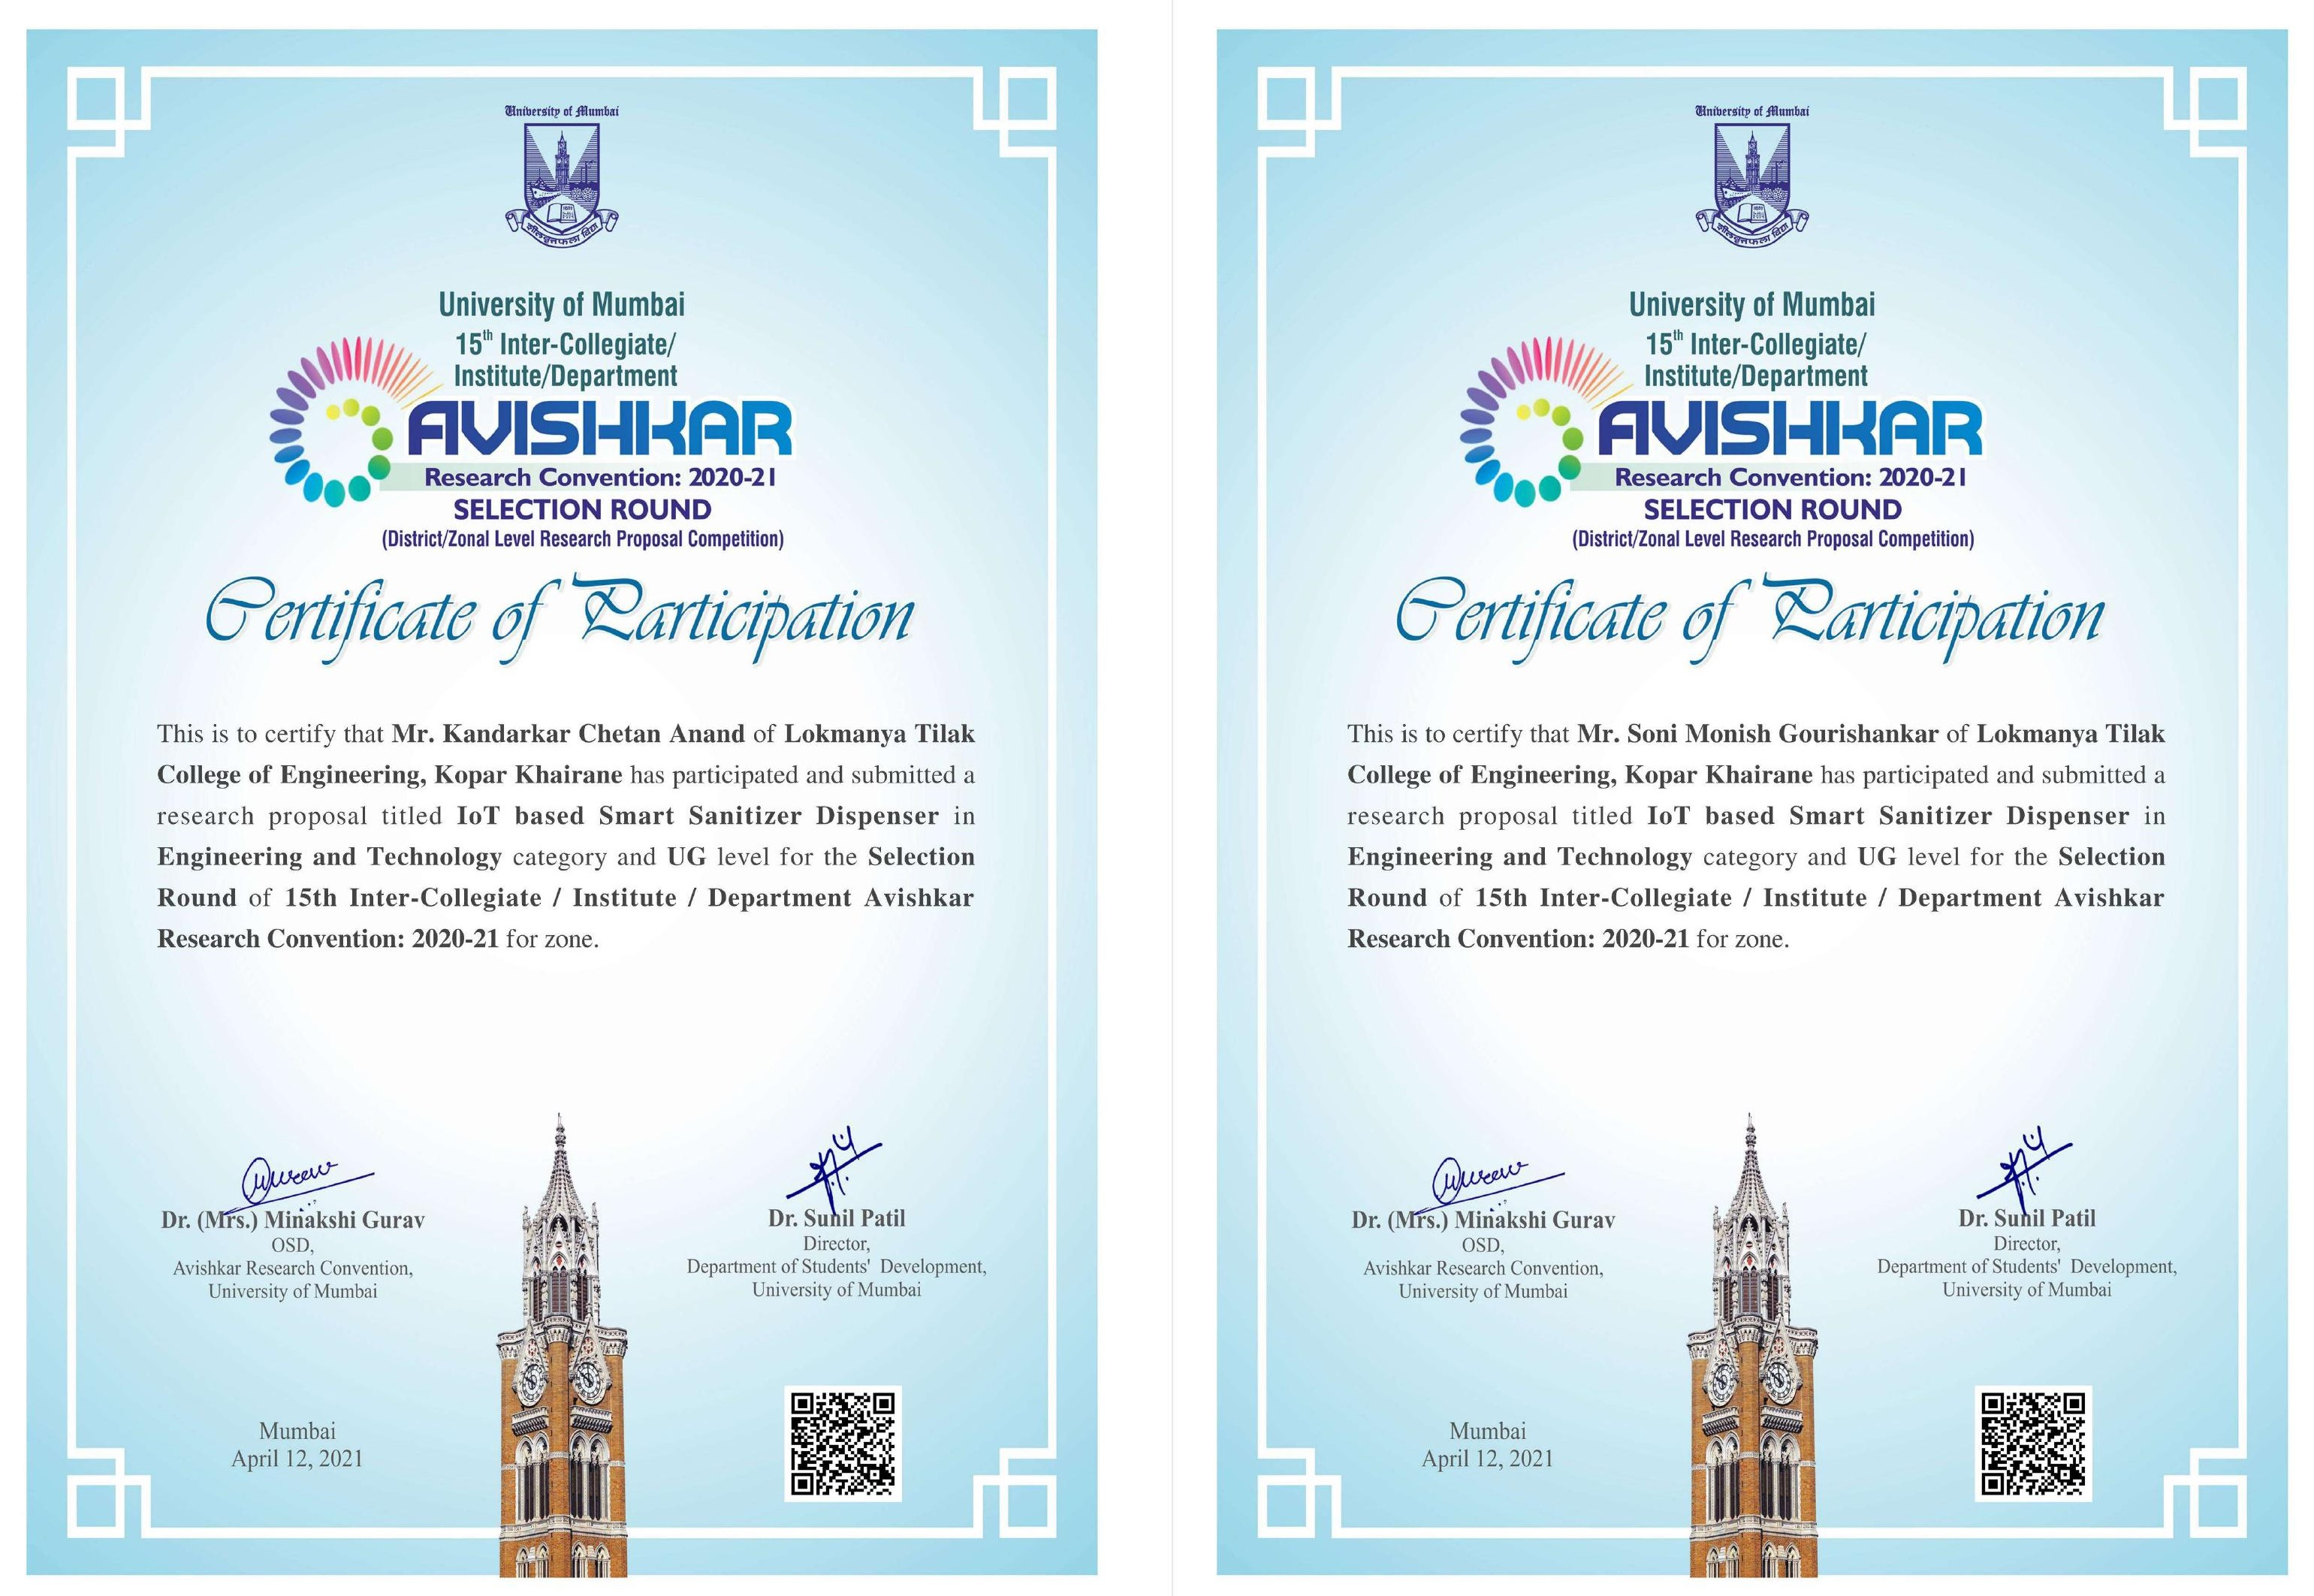
\includegraphics[width=140mm,scale=1]{certi1}
\end{figure}

\newpage

\vspace{3cm}
   \begin{figure}[h]
		\centering
	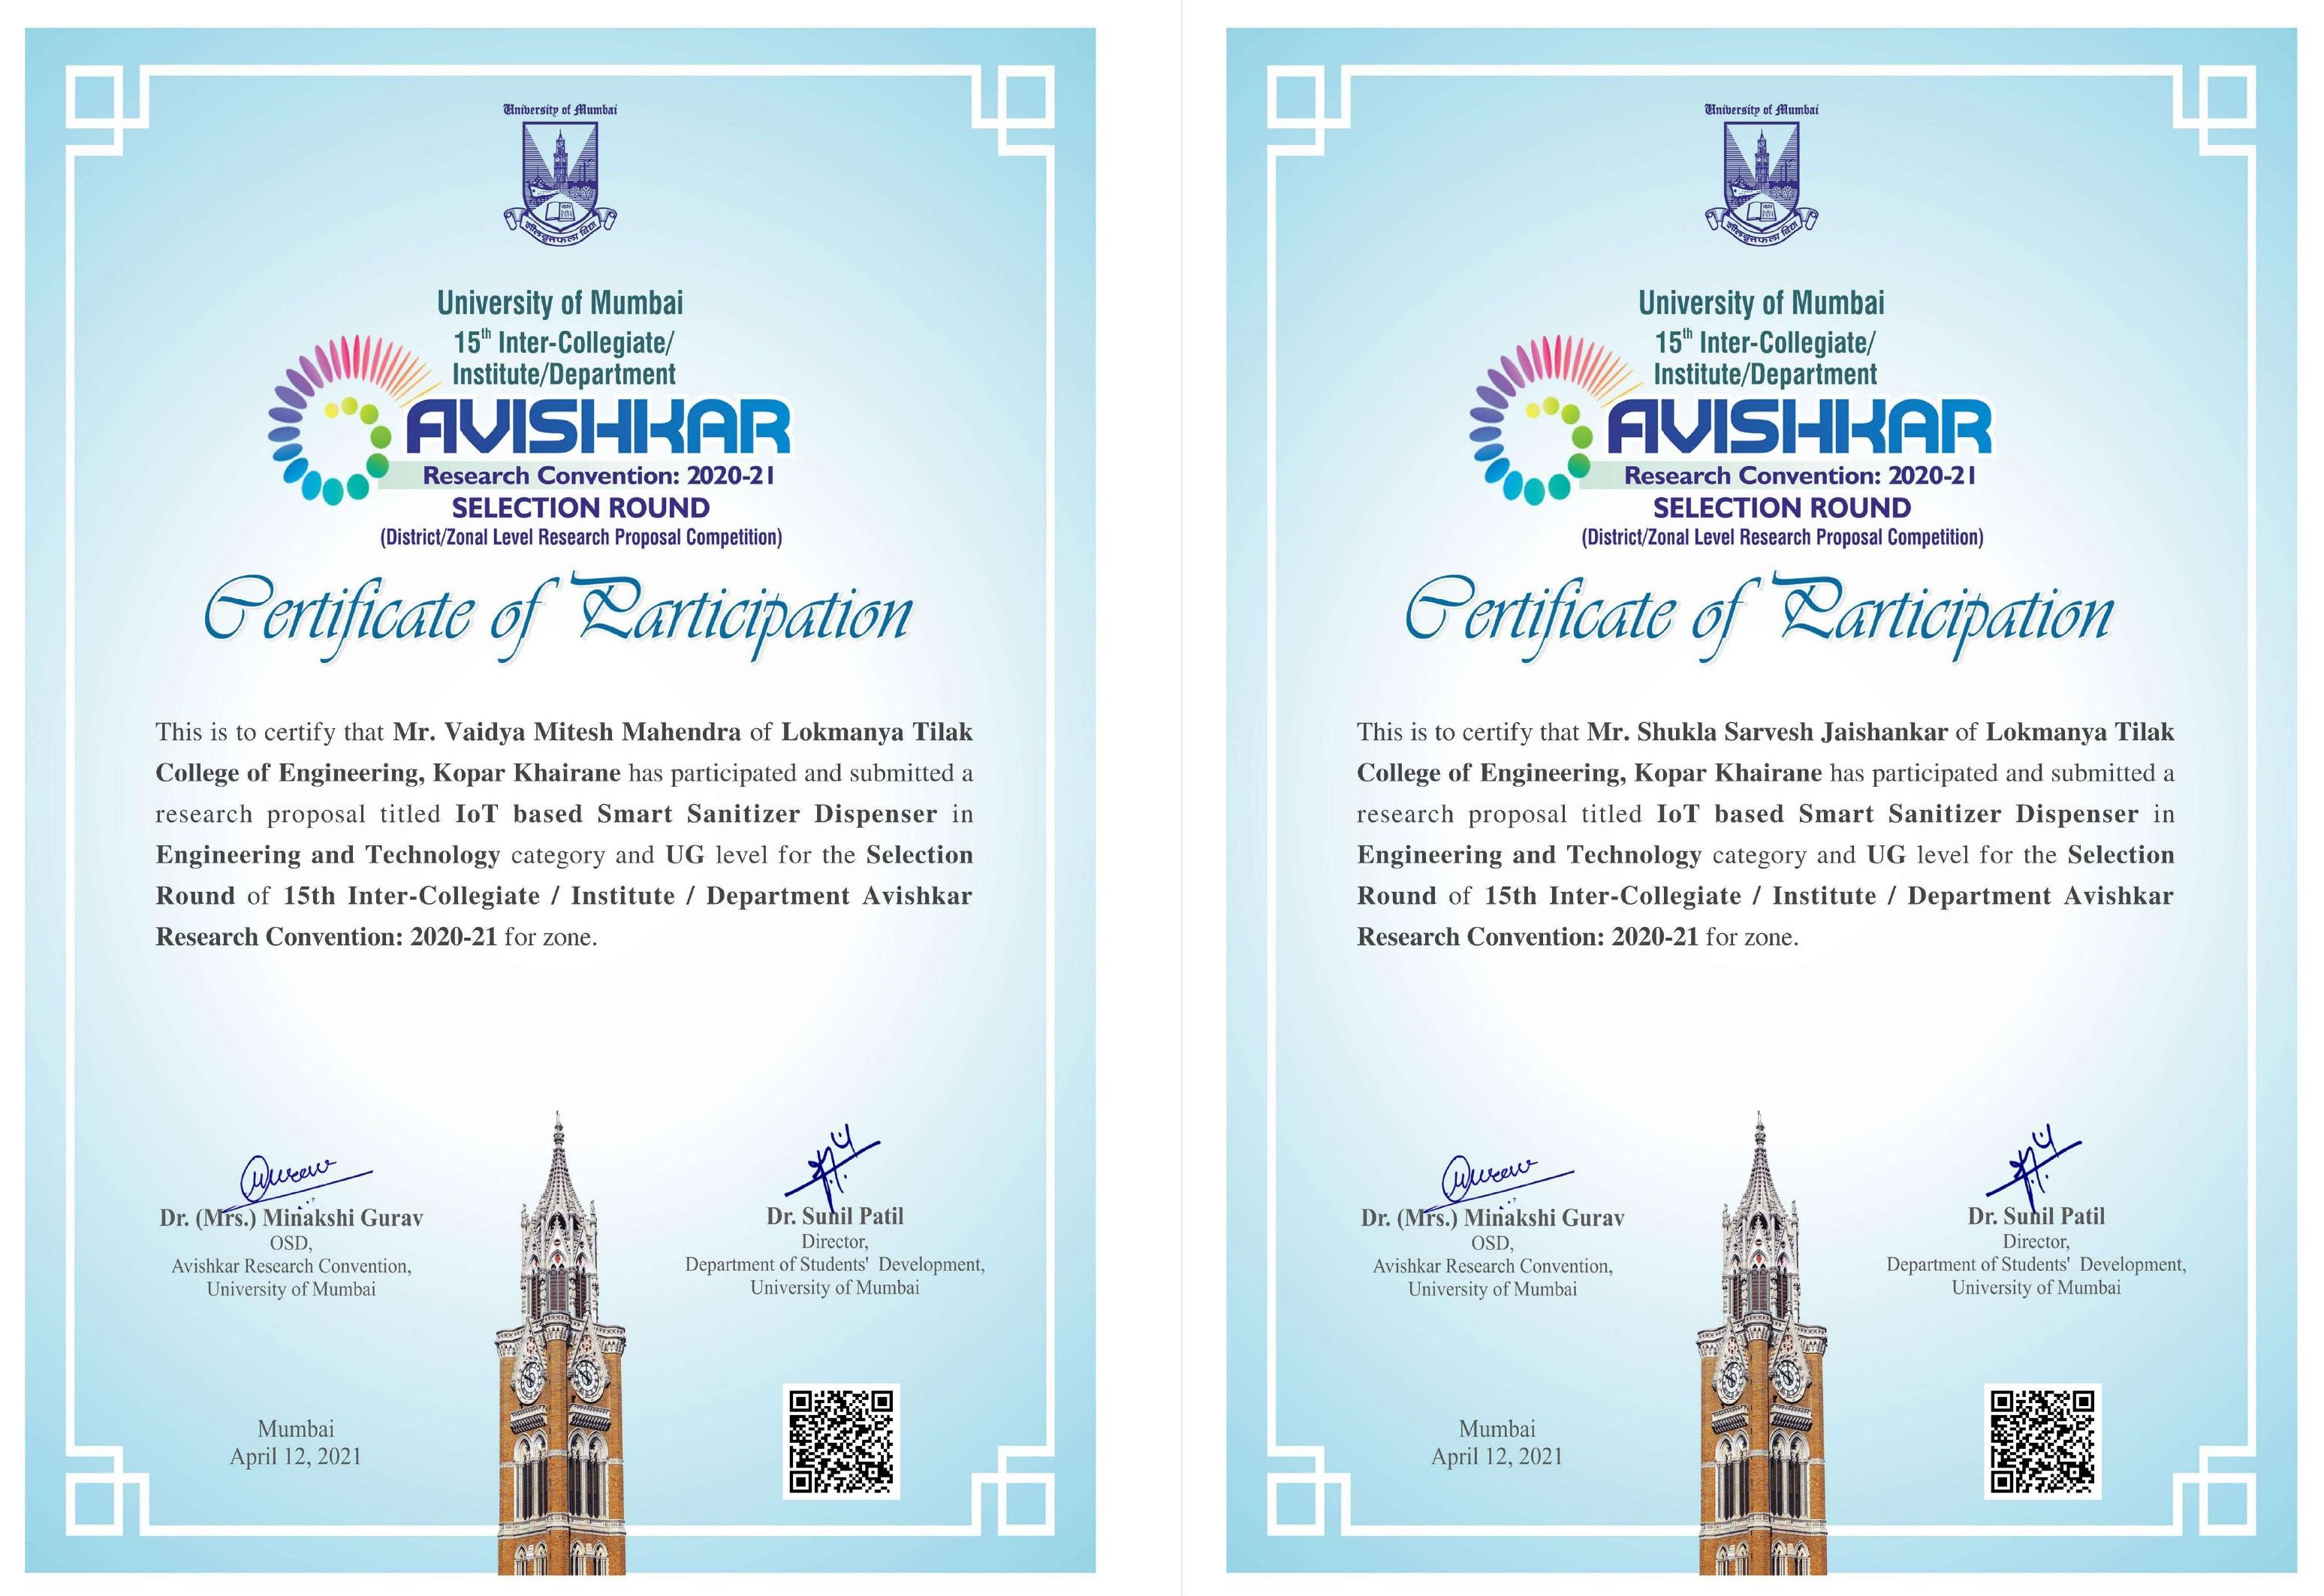
\includegraphics[width=140mm,scale=1]{certi2}
\end{figure}
 
 \vspace{1cm}

\newpage 
   \begin{flushleft}	 
	\hspace{0.5cm} \large \textbf{Anveshana Certificates} 
	\vspace{0.5cm} 
	\end{flushleft} 


   \begin{figure}[h]
		\centering
	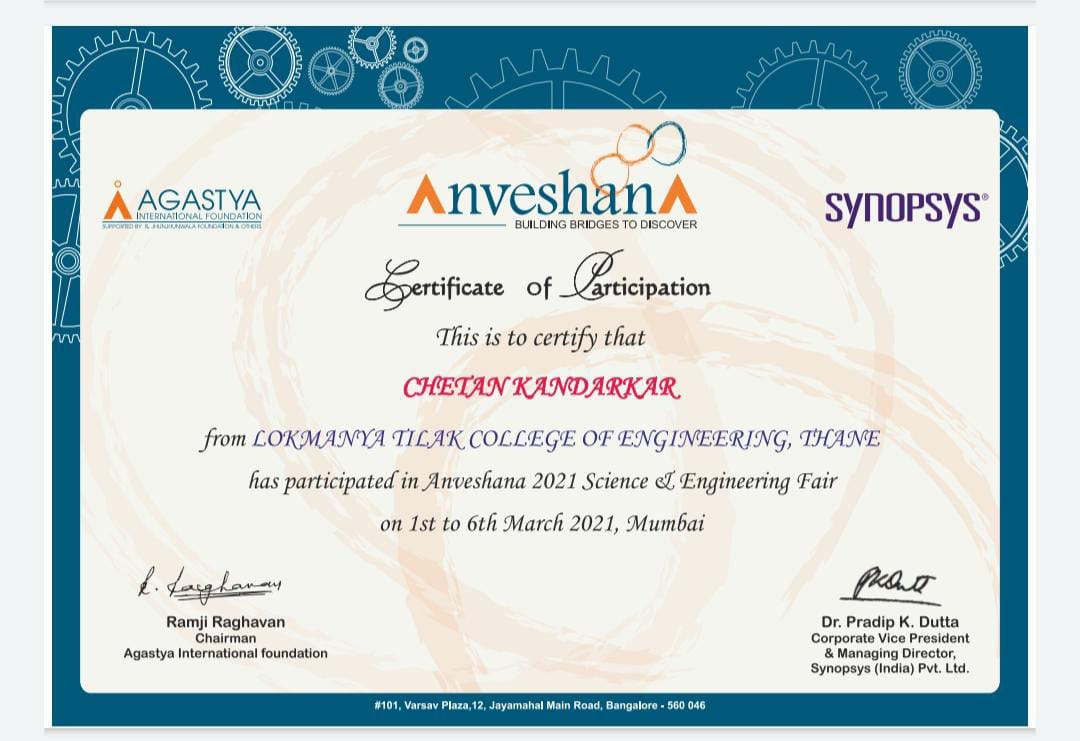
\includegraphics[width=100mm,scale=1]{chetan2}
\end{figure}

\vspace{1cm}

\begin{figure}[h]
    \centering
    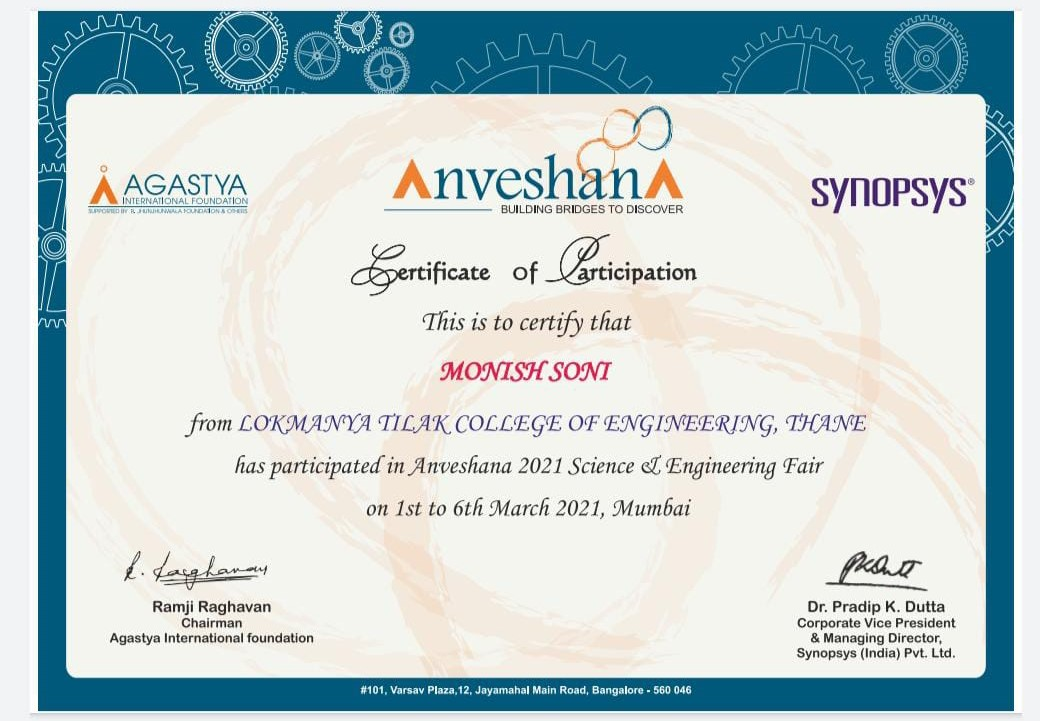
\includegraphics[width=100mm,scale=1]{monish2}
\end{figure}

\newpage

\vspace{1cm}

   \begin{figure}[h]
		\centering
	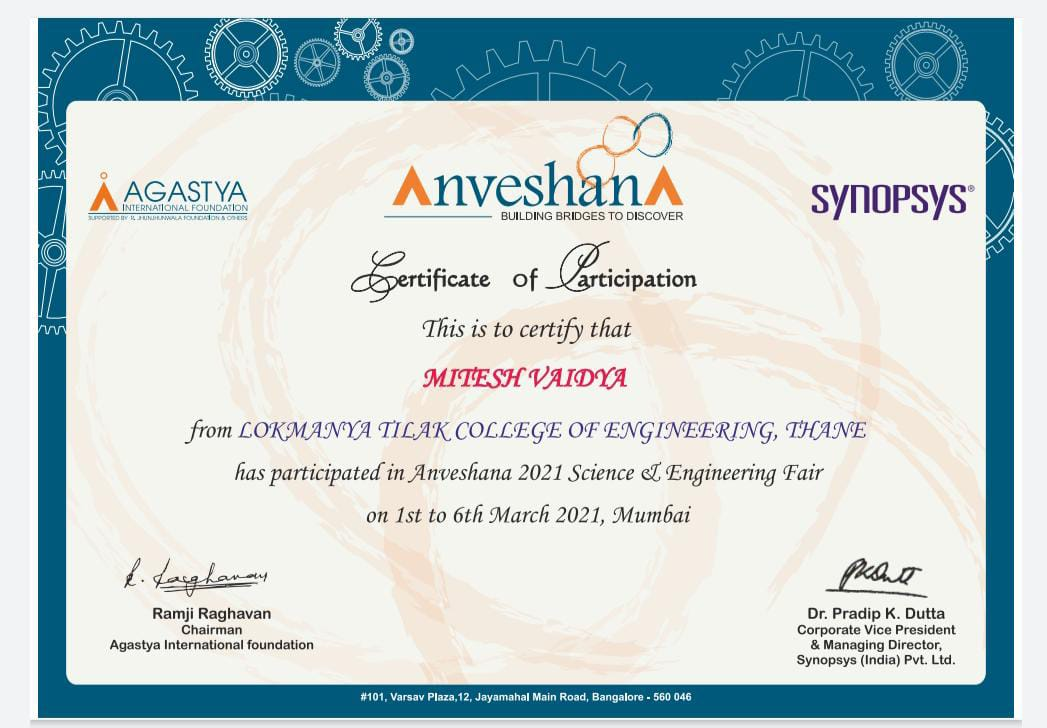
\includegraphics[width=100mm,scale=1]{mitesh2}
\end{figure}

\vspace{1cm}

\begin{figure}[h]
    \centering
    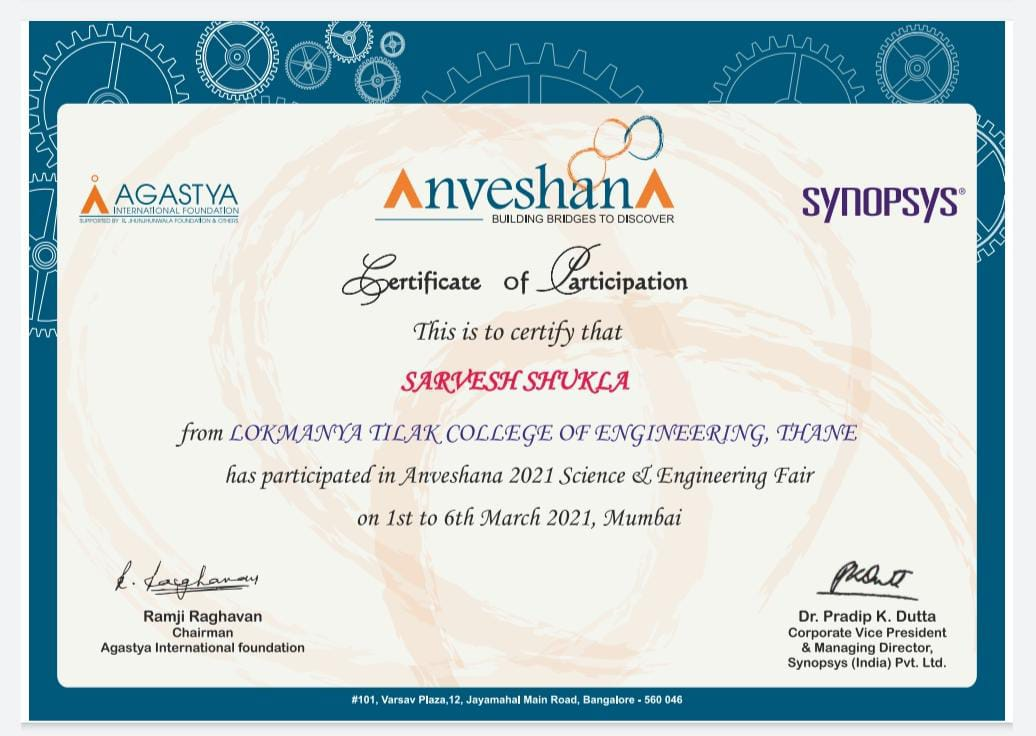
\includegraphics[width=100mm,scale=1]{sarvesh2}
\end{figure}

 



%\renewcommand{\bibname}{References}

%\bibliographystyle{plain}
%\bibliographystyle{plainnat}
%\bibliographystyle{agsm}

%\bibliography{database}
%\renewcommand{\bibliography}{\References}
%\addcontentsline{toc}{chapter}{References}


\end{document}

